\chapter{Análisis Conceptual (CIM)}

\section{El Modelo Independiente de Computación}

El Análisis Conceptual representa el nivel superior en la abstracción \textit{MDAA}. En esta fase, el usuario define el \textit{CIM} (\textit{Computation Independent Model}), centrándose exclusivamente en los requerimientos lógicos del dominio musical, sin considerar aún aspectos tecnológicos de su futura implementación.

\begin{figure}[!ht]
    \centering
    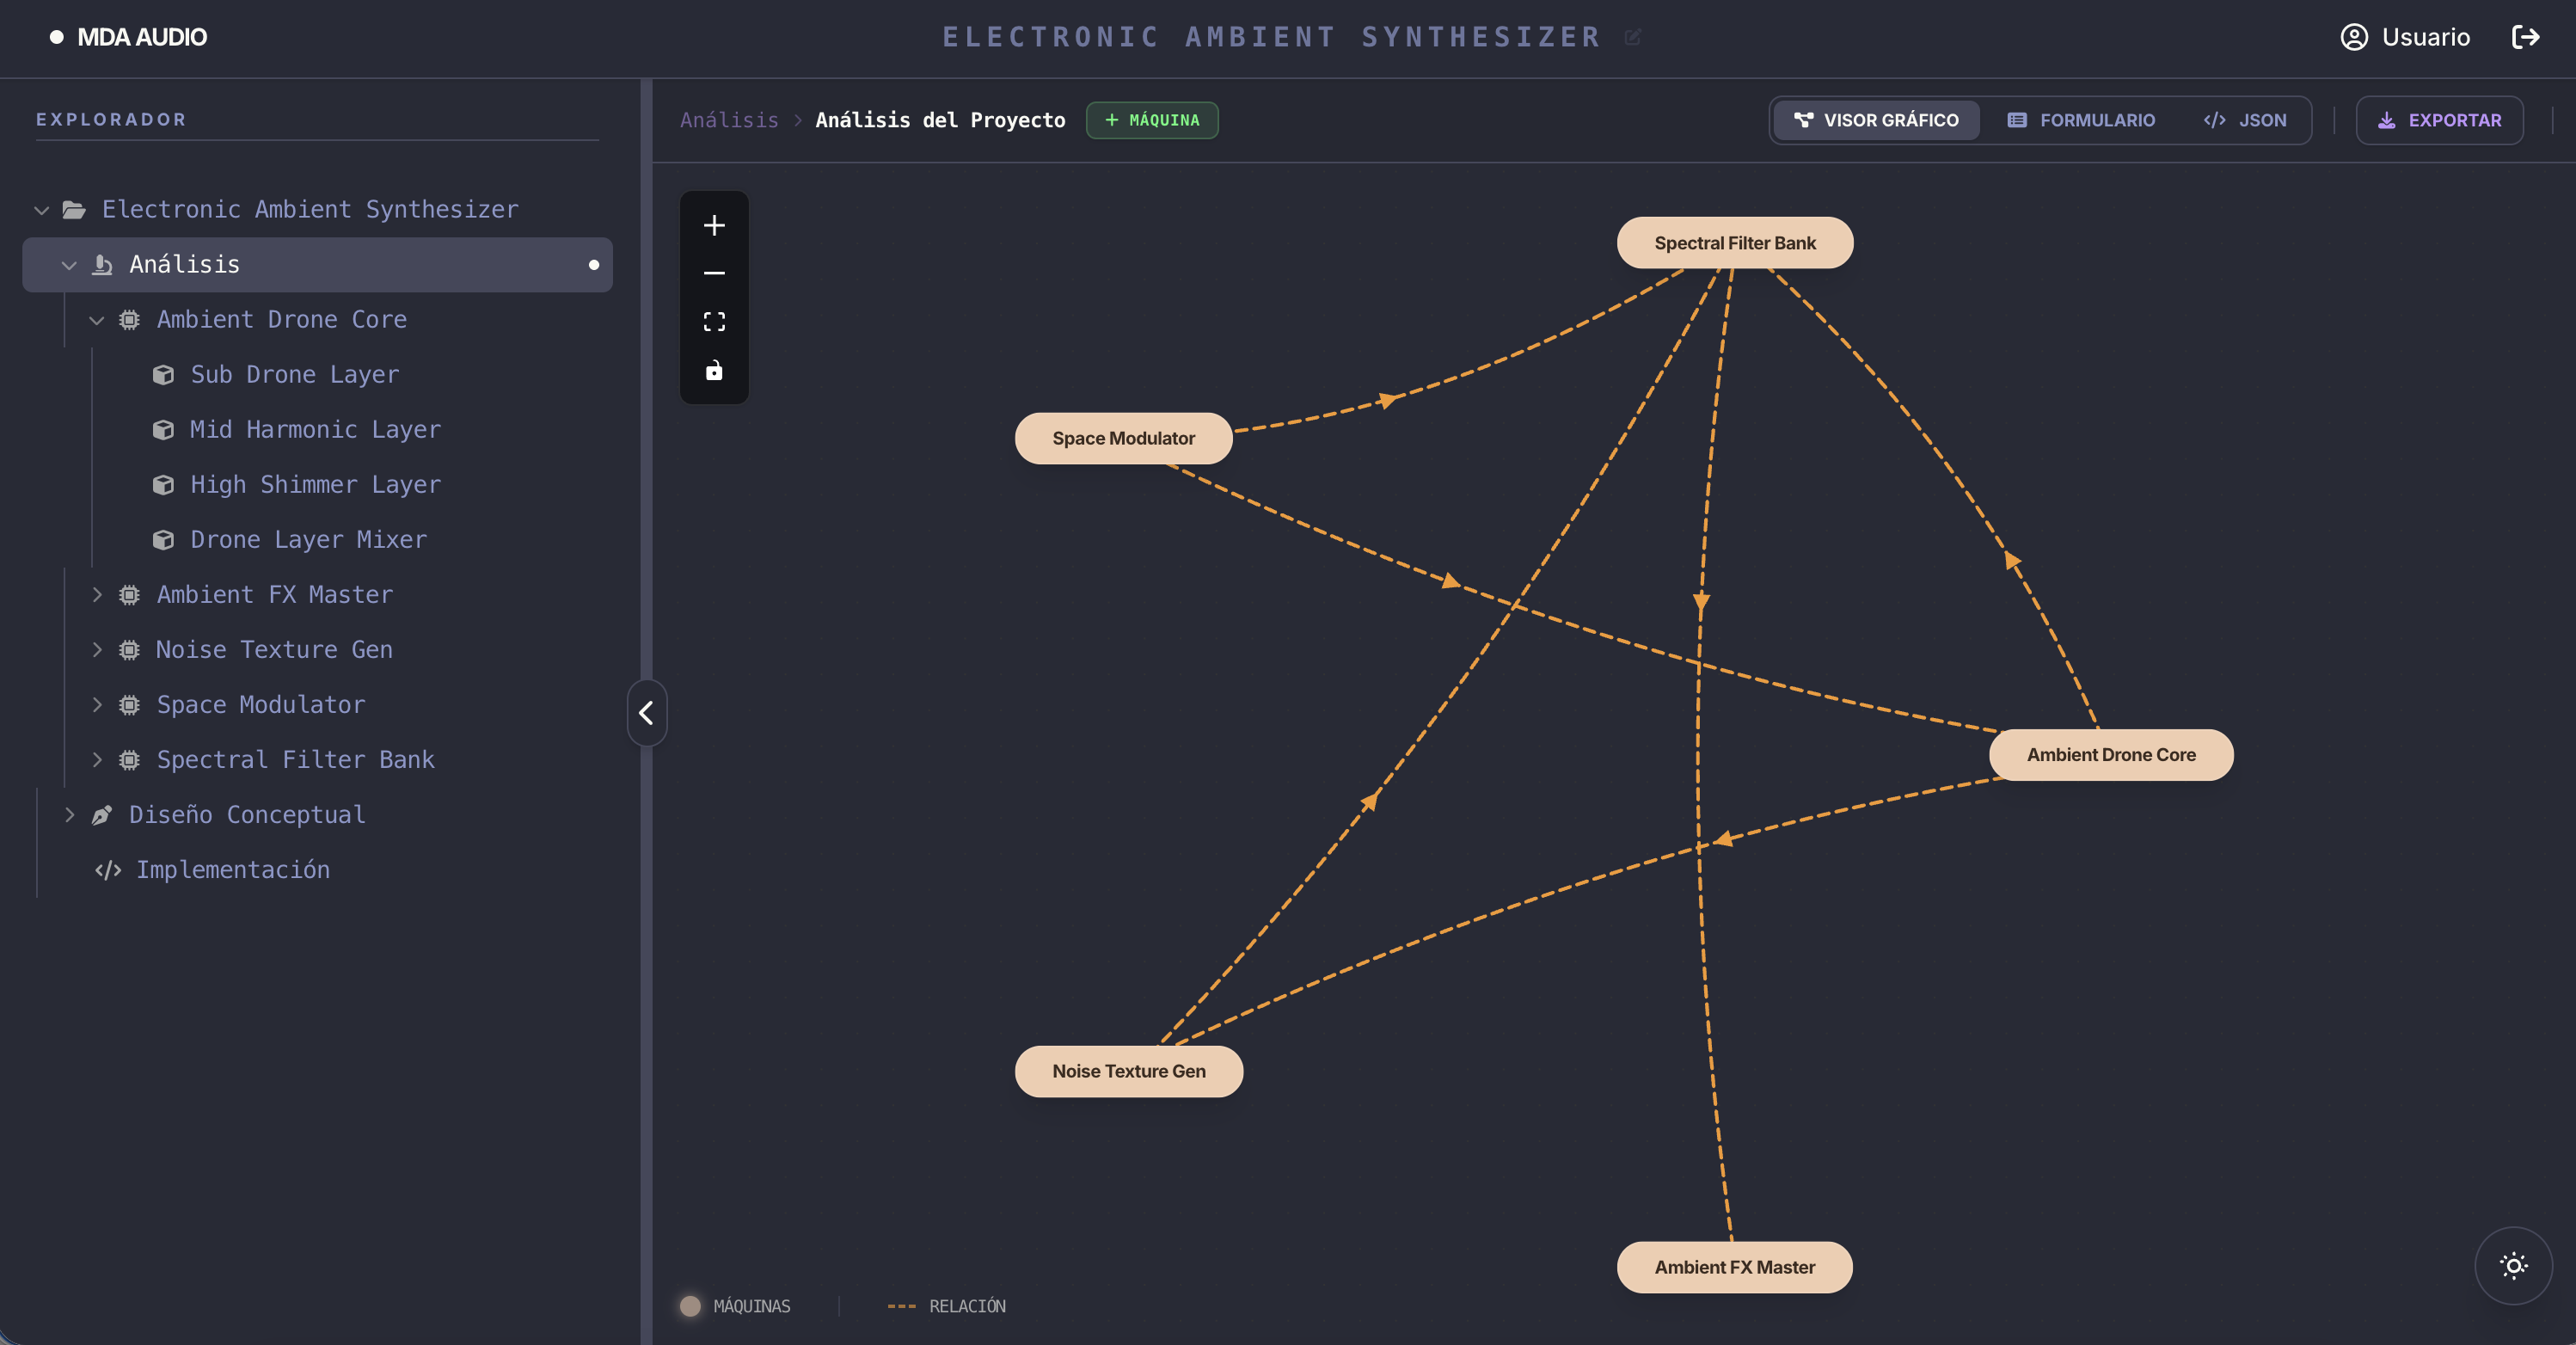
\includegraphics[width=\textwidth]{imagenes/05_analisis/01_pantallaPrincipalAnalisis.png}
    \caption{Vista general del entorno de Análisis Conceptual.}
\end{figure}

Al seleccionar la rama de Análisis Conceptual en el explorador, se abre el área de trabajo dedicada al entorno \textit{CIM}. Esta interfaz facilita la gestión de las entidades principales (las máquinas conceptuales) y la definición de las interacciones lógicas entre ellas.

\begin{figure}[!ht]
    \centering
    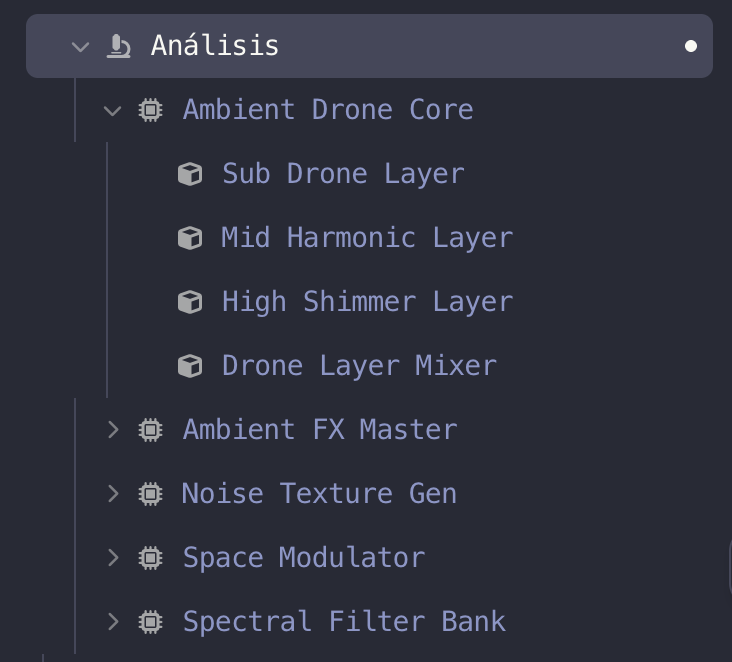
\includegraphics[width=0.4\textwidth]{imagenes/05_analisis/02_exploradorAnalisis.png}
    \caption{Detalle del nodo de Análisis Conceptual en el explorador.}
\end{figure}

El nodo raíz de \textit{CIM} actúa como contenedor global. Desplegando esta rama, el usuario puede navegar hacia la configuración orquestal (relaciones) o acceder a la definición específica de cada máquina conceptual individual.

\begin{figure}[!ht]
    \centering
    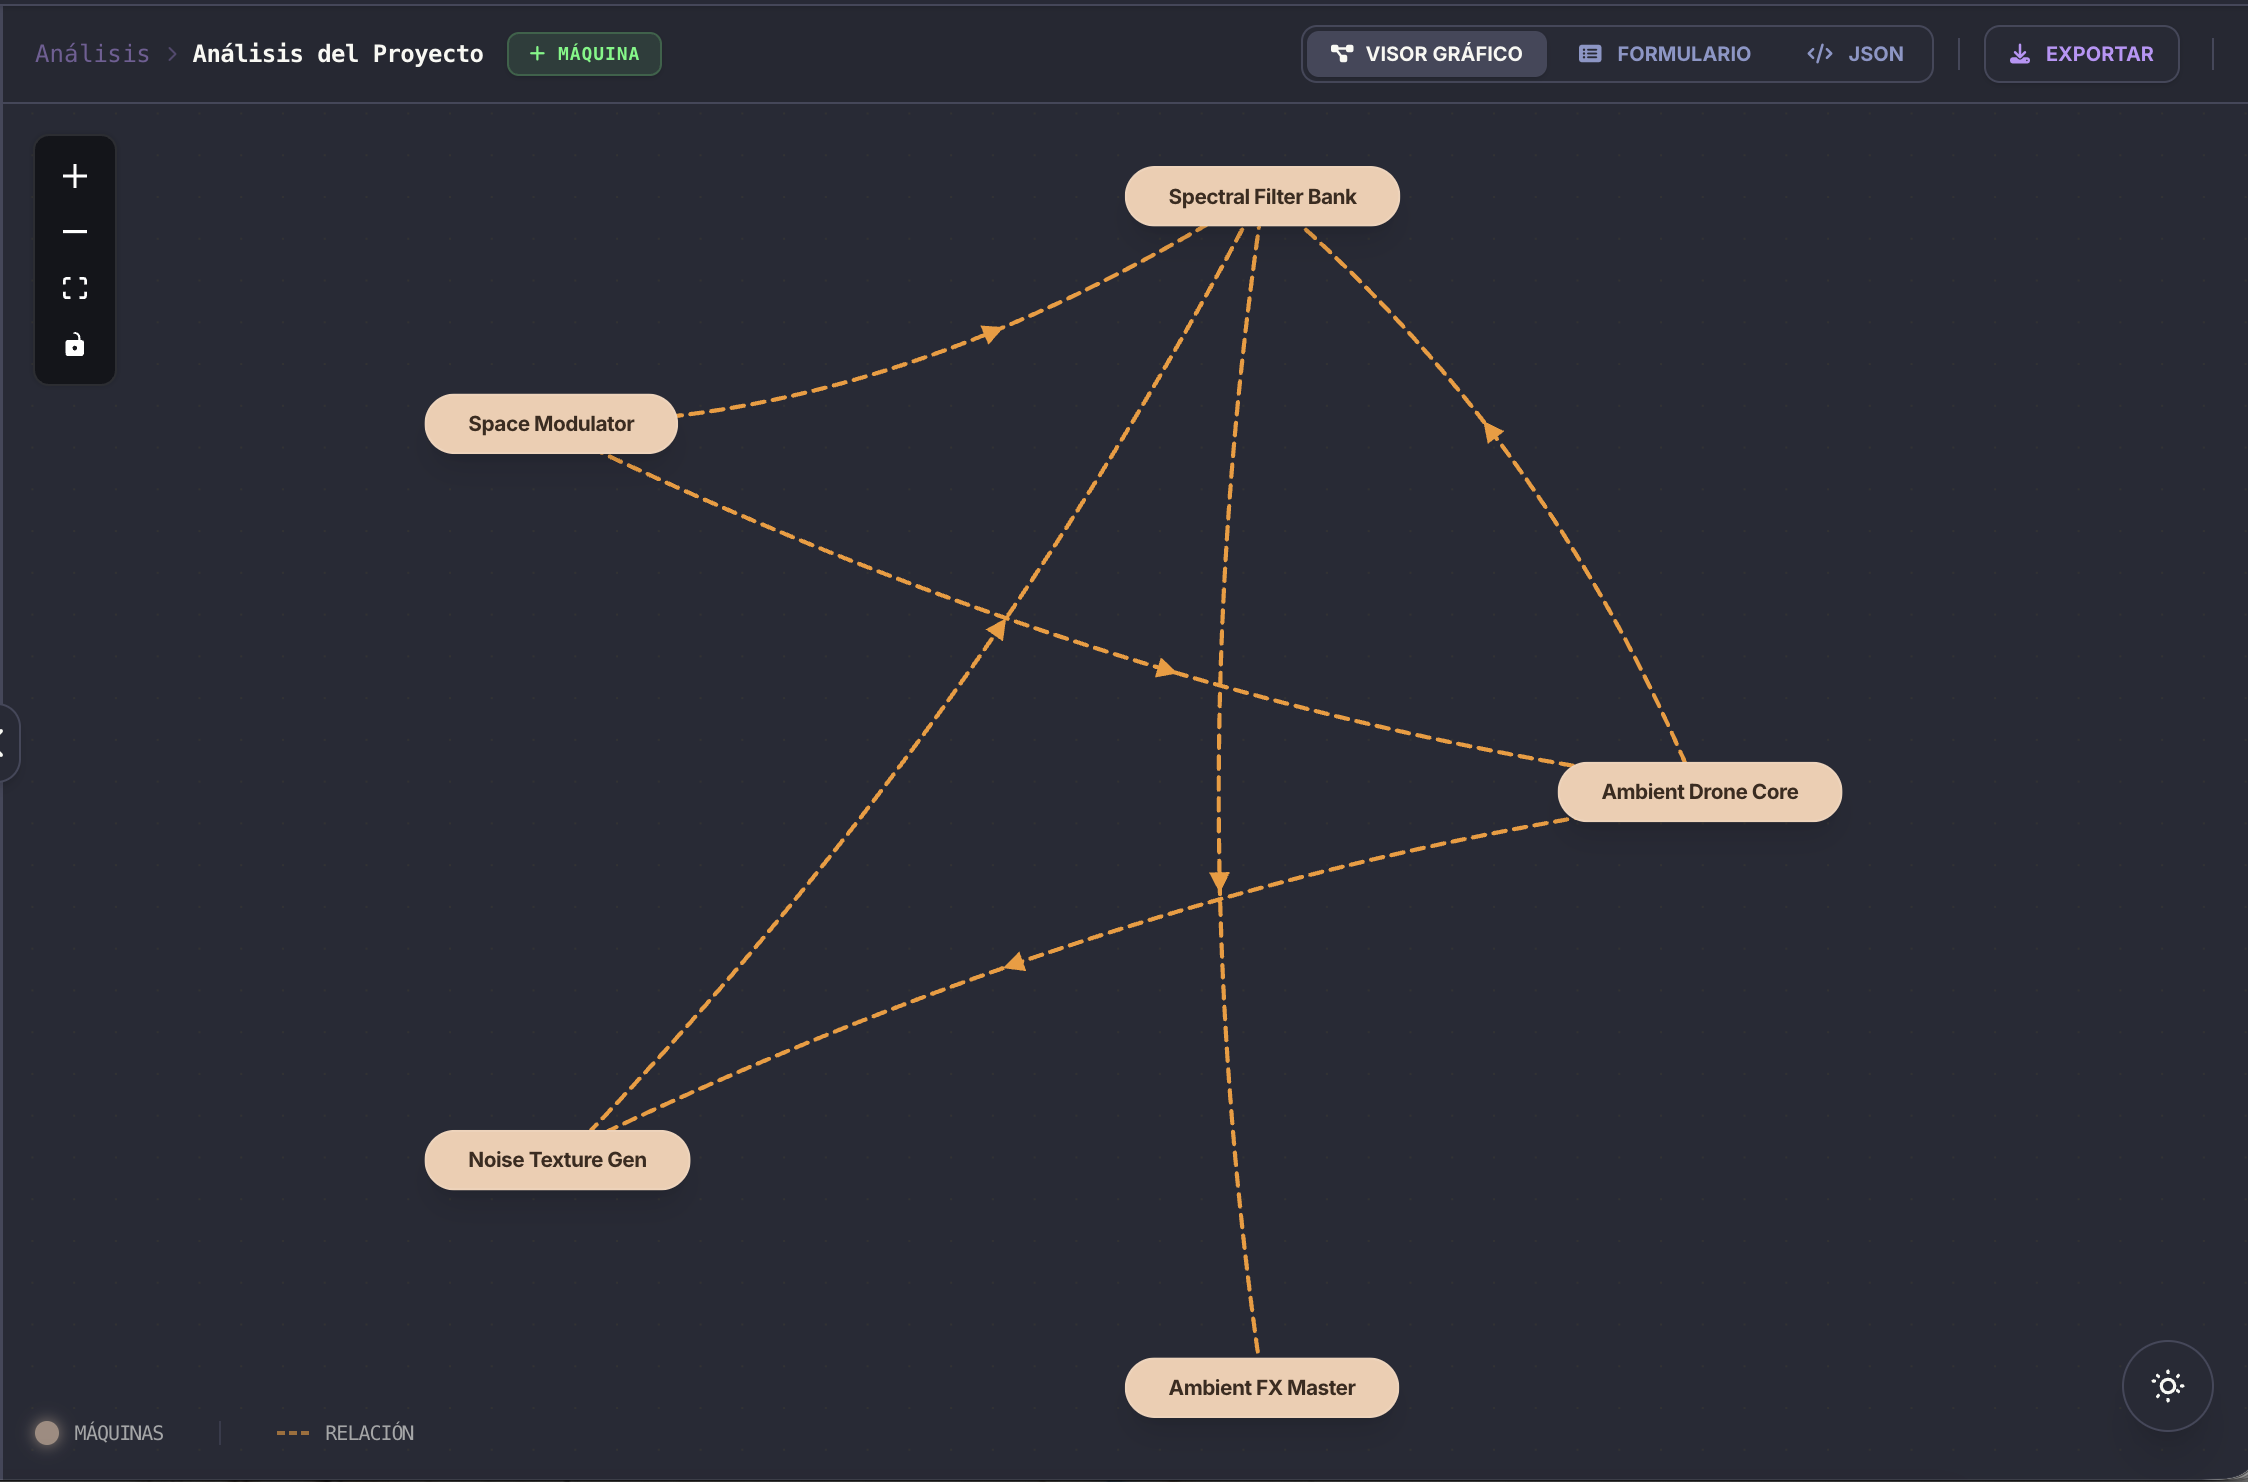
\includegraphics[width=\textwidth]{imagenes/05_analisis/03_pantallaVistaDelNodoAnalisis.png}
    \caption{Pantalla de vista detallada al seleccionar el nodo raíz de Análisis Conceptual.}
\end{figure}

La pantalla principal del nivel \textit{CIM} centraliza las herramientas para la gestión estructural. Su propósito es definir la red de componentes musicales.

\subsection{Creación de Máquinas Conceptuales}

\begin{figure}[!ht]
    \centering
    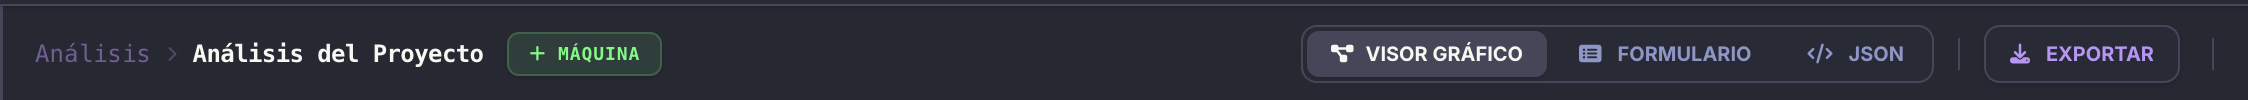
\includegraphics[width=0.4\textwidth]{imagenes/05_analisis/04_botoneraAccionAnalisis.png}
    \caption{Botonera de acciones globales del Análisis Conceptual.}
\end{figure}

\begin{figure}[!ht]
    \centering
    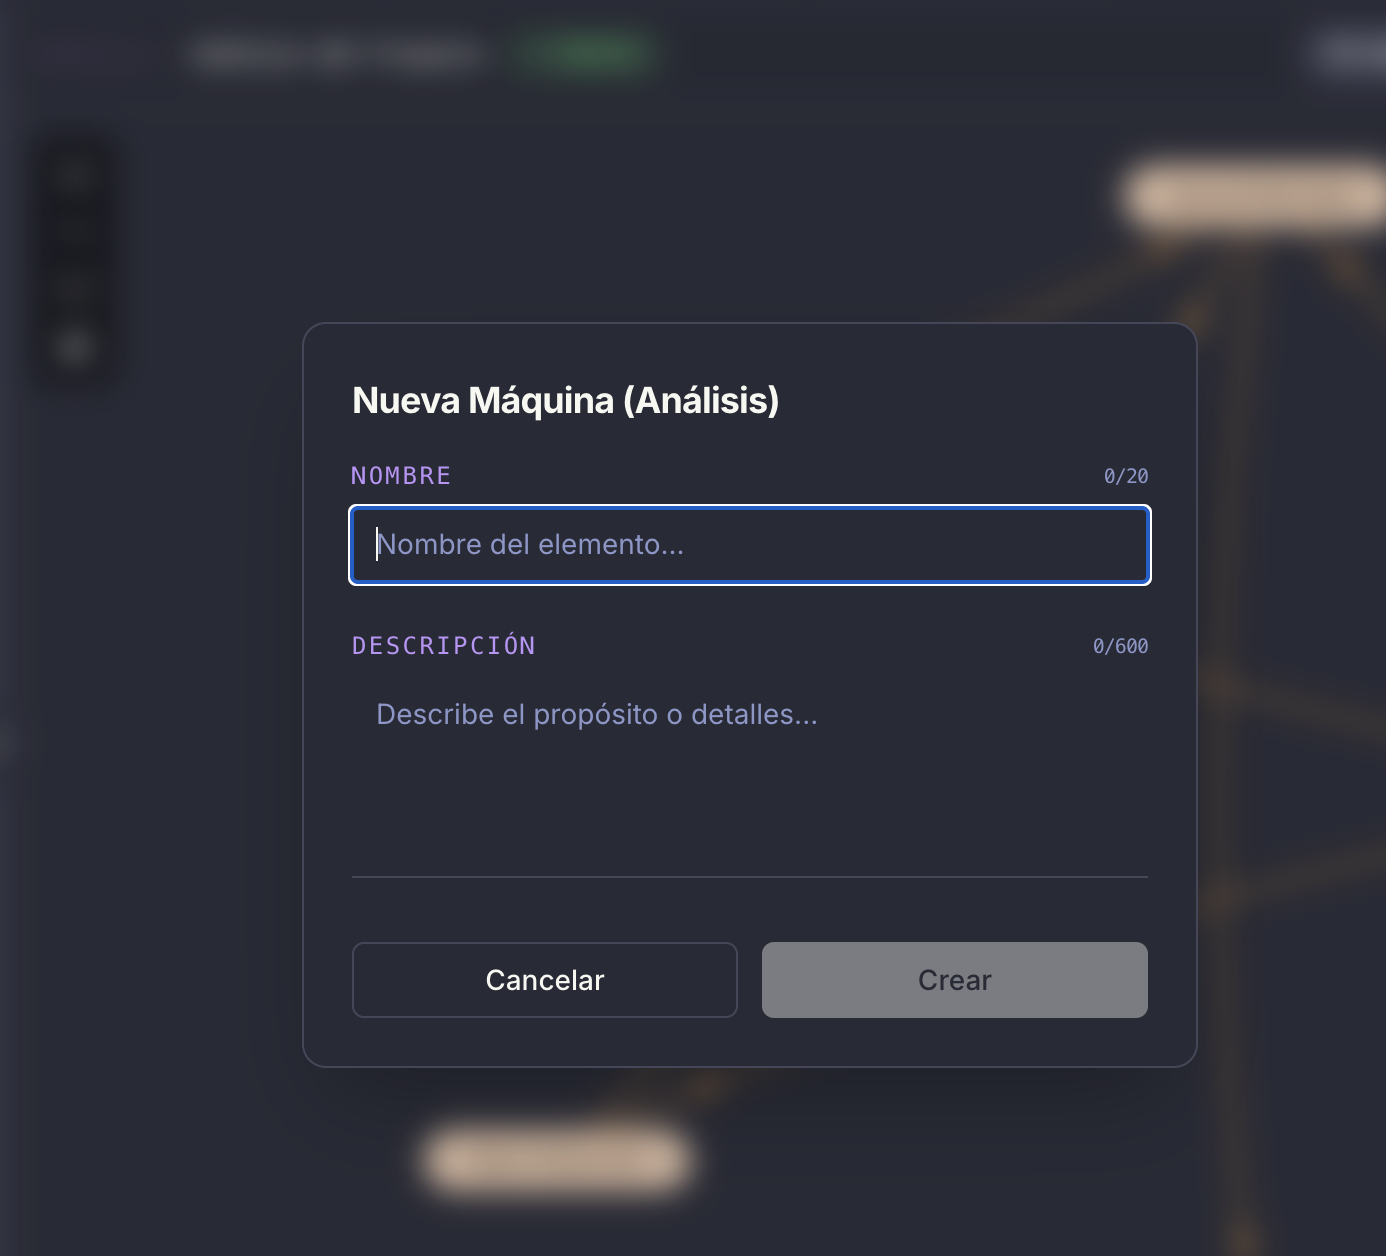
\includegraphics[width=0.6\textwidth]{imagenes/05_analisis/05_crearMaquina.png}
    \caption{Formulario para la creación de una nueva máquina CIM.}
\end{figure}

Desde la botonera superior es posible invocar la creación de nuevas máquinas. Este formulario solicita información esencial, como el identificador único, para instanciar el elemento dentro del modelo del lenguaje \textit{DSL}. Una vez salvada, la nueva máquina se incorpora al árbol del explorador.

\section{Gestión de Relaciones CIM}

Para establecer la conectividad conceptual entre las máquinas, la plataforma ofrece tres modos de trabajo adaptados a distintos perfiles de usuario.

\begin{figure}[!ht]
    \centering
    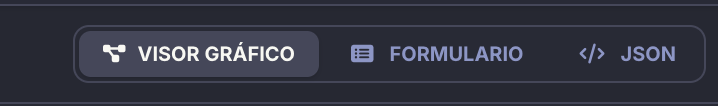
\includegraphics[width=0.5\textwidth]{imagenes/05_analisis/06_botoneraVistasAnalisis.png}
    \caption{Selector de vistas: Visor Gráfico, Formulario y Código JSON.}
\end{figure}

La botonera de vistas permite alternar instantáneamente entre la representación gráfica, el editor basado en formularios y el editor de código avanzado.

\subsection{Visor Gráfico}

\begin{figure}[!ht]
    \centering
    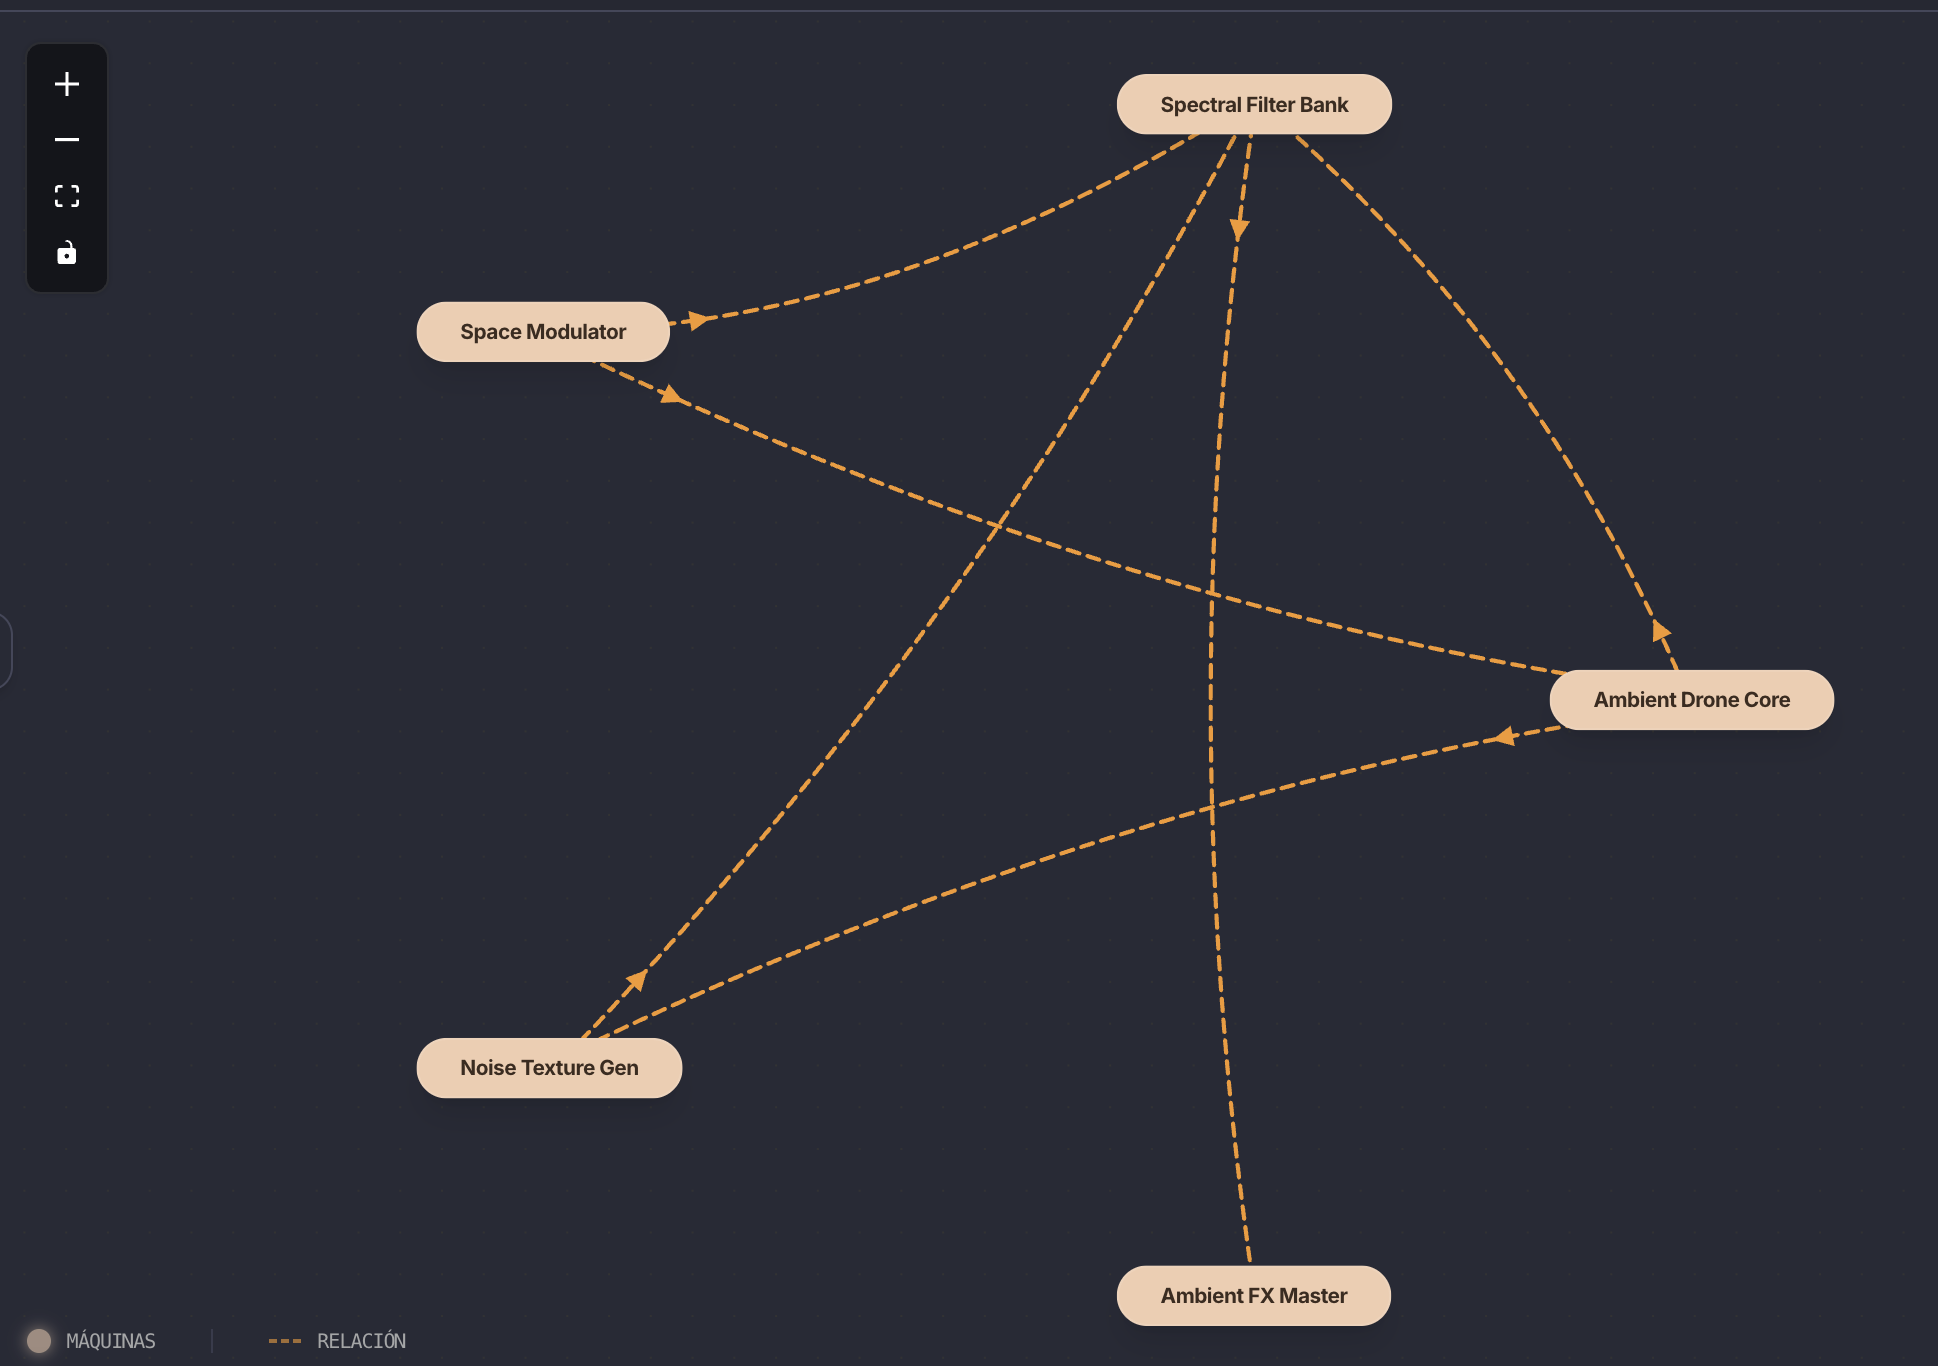
\includegraphics[width=\textwidth]{imagenes/05_analisis/07_grafoRelacionesAnalisis.png}
    \caption{Representación en forma de grafo interactivo de las relaciones entre máquinas.}
\end{figure}

El visor muestra un grafo dinámico. Los nodos simbolizan las máquinas conceptuales, mientras que las aristas direccionadas exponen el flujo de la señal o la lógica de control.

\begin{figure}[!ht]
    \centering
    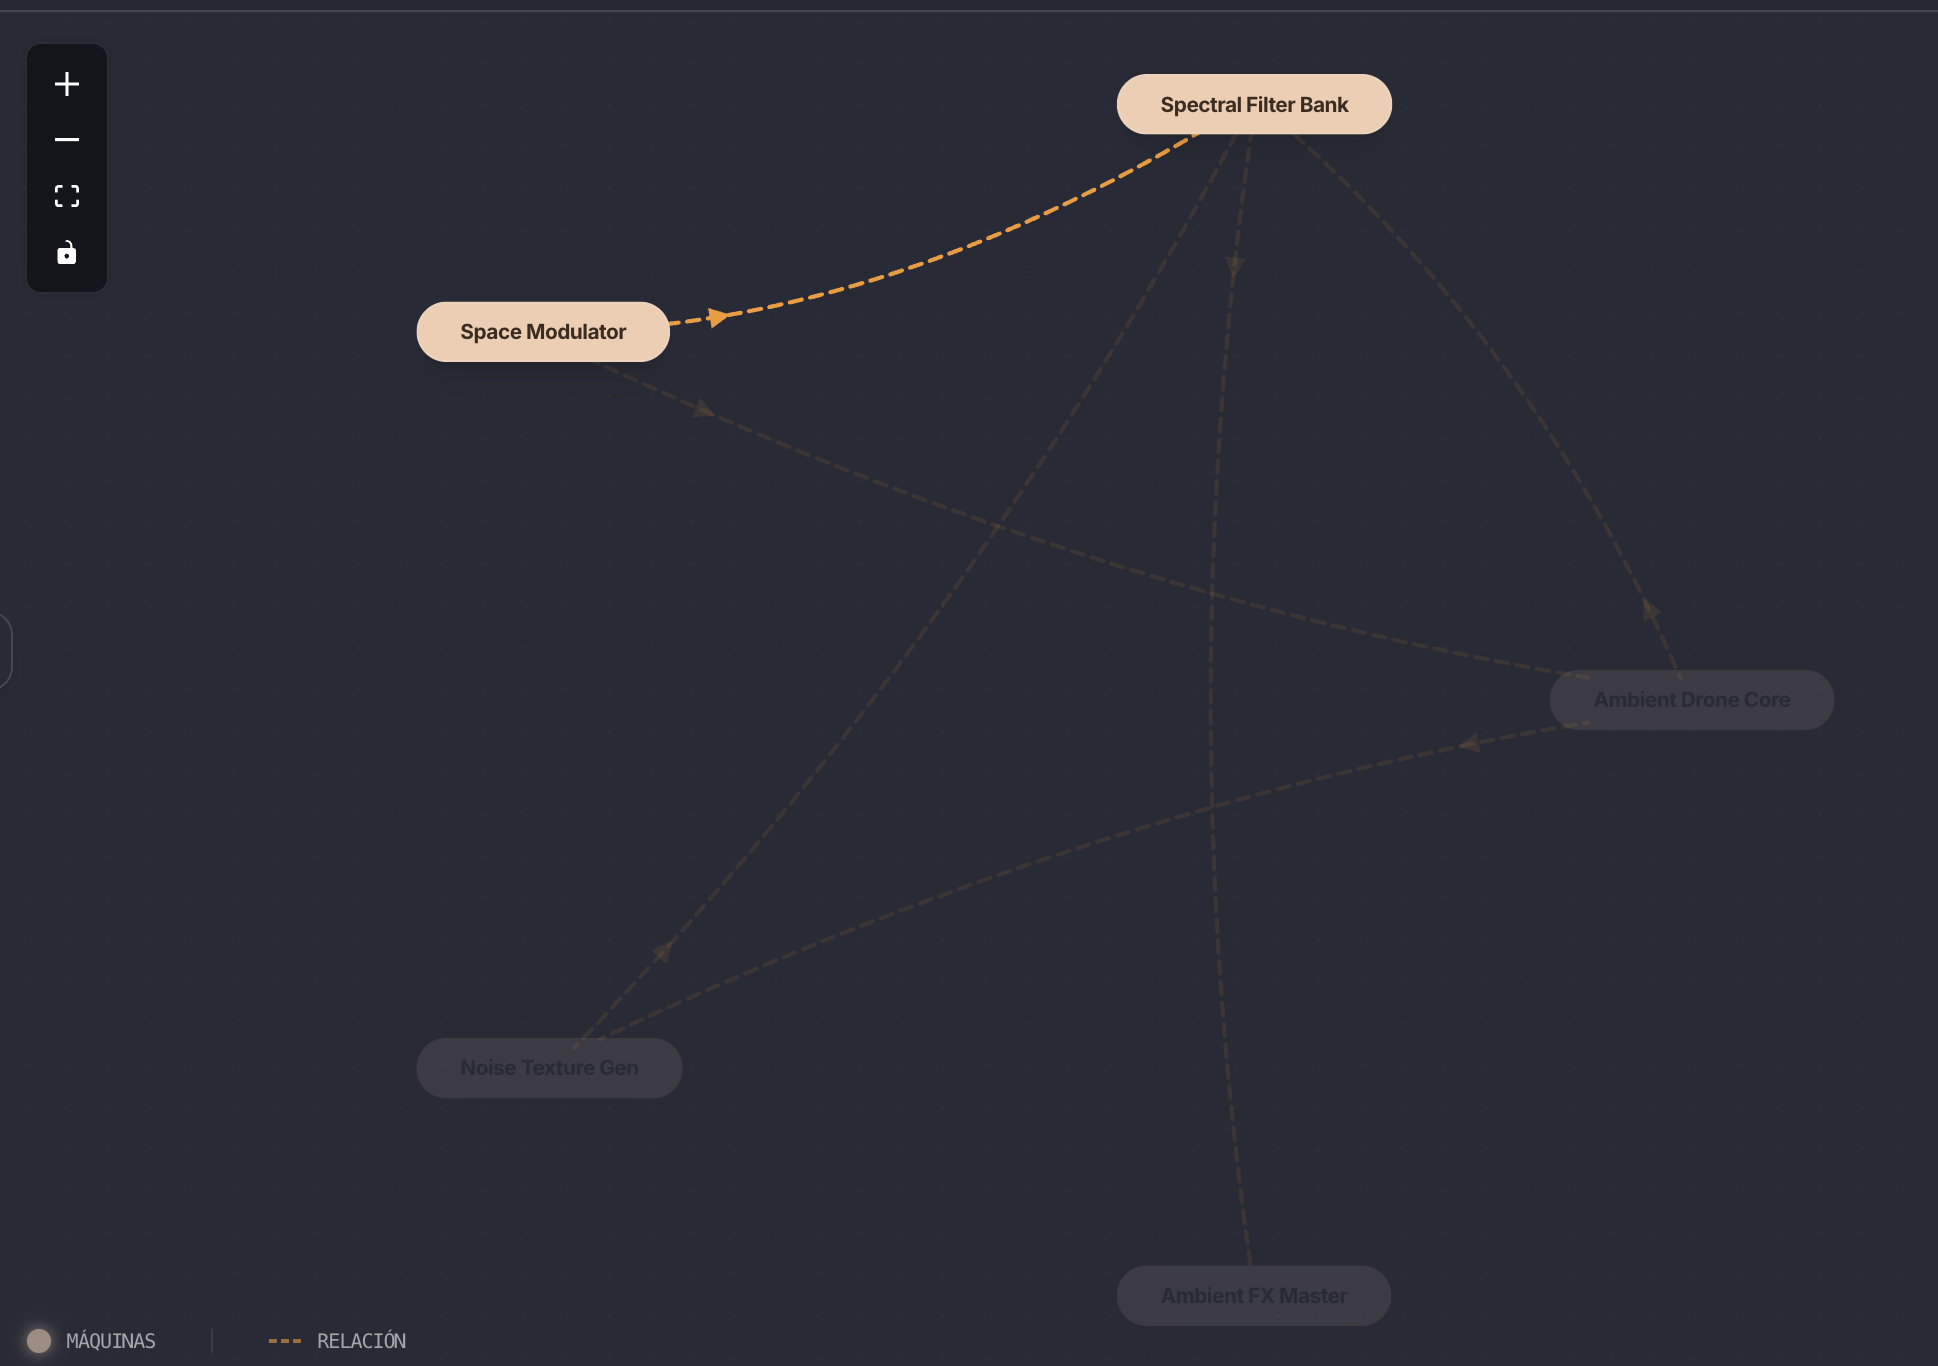
\includegraphics[width=\textwidth]{imagenes/05_analisis/08_aristaGrafoPulsado.png}
    \caption{Inspección de metadatos al seleccionar una relación (arista).}
\end{figure}

\begin{figure}[!ht]
    \centering
    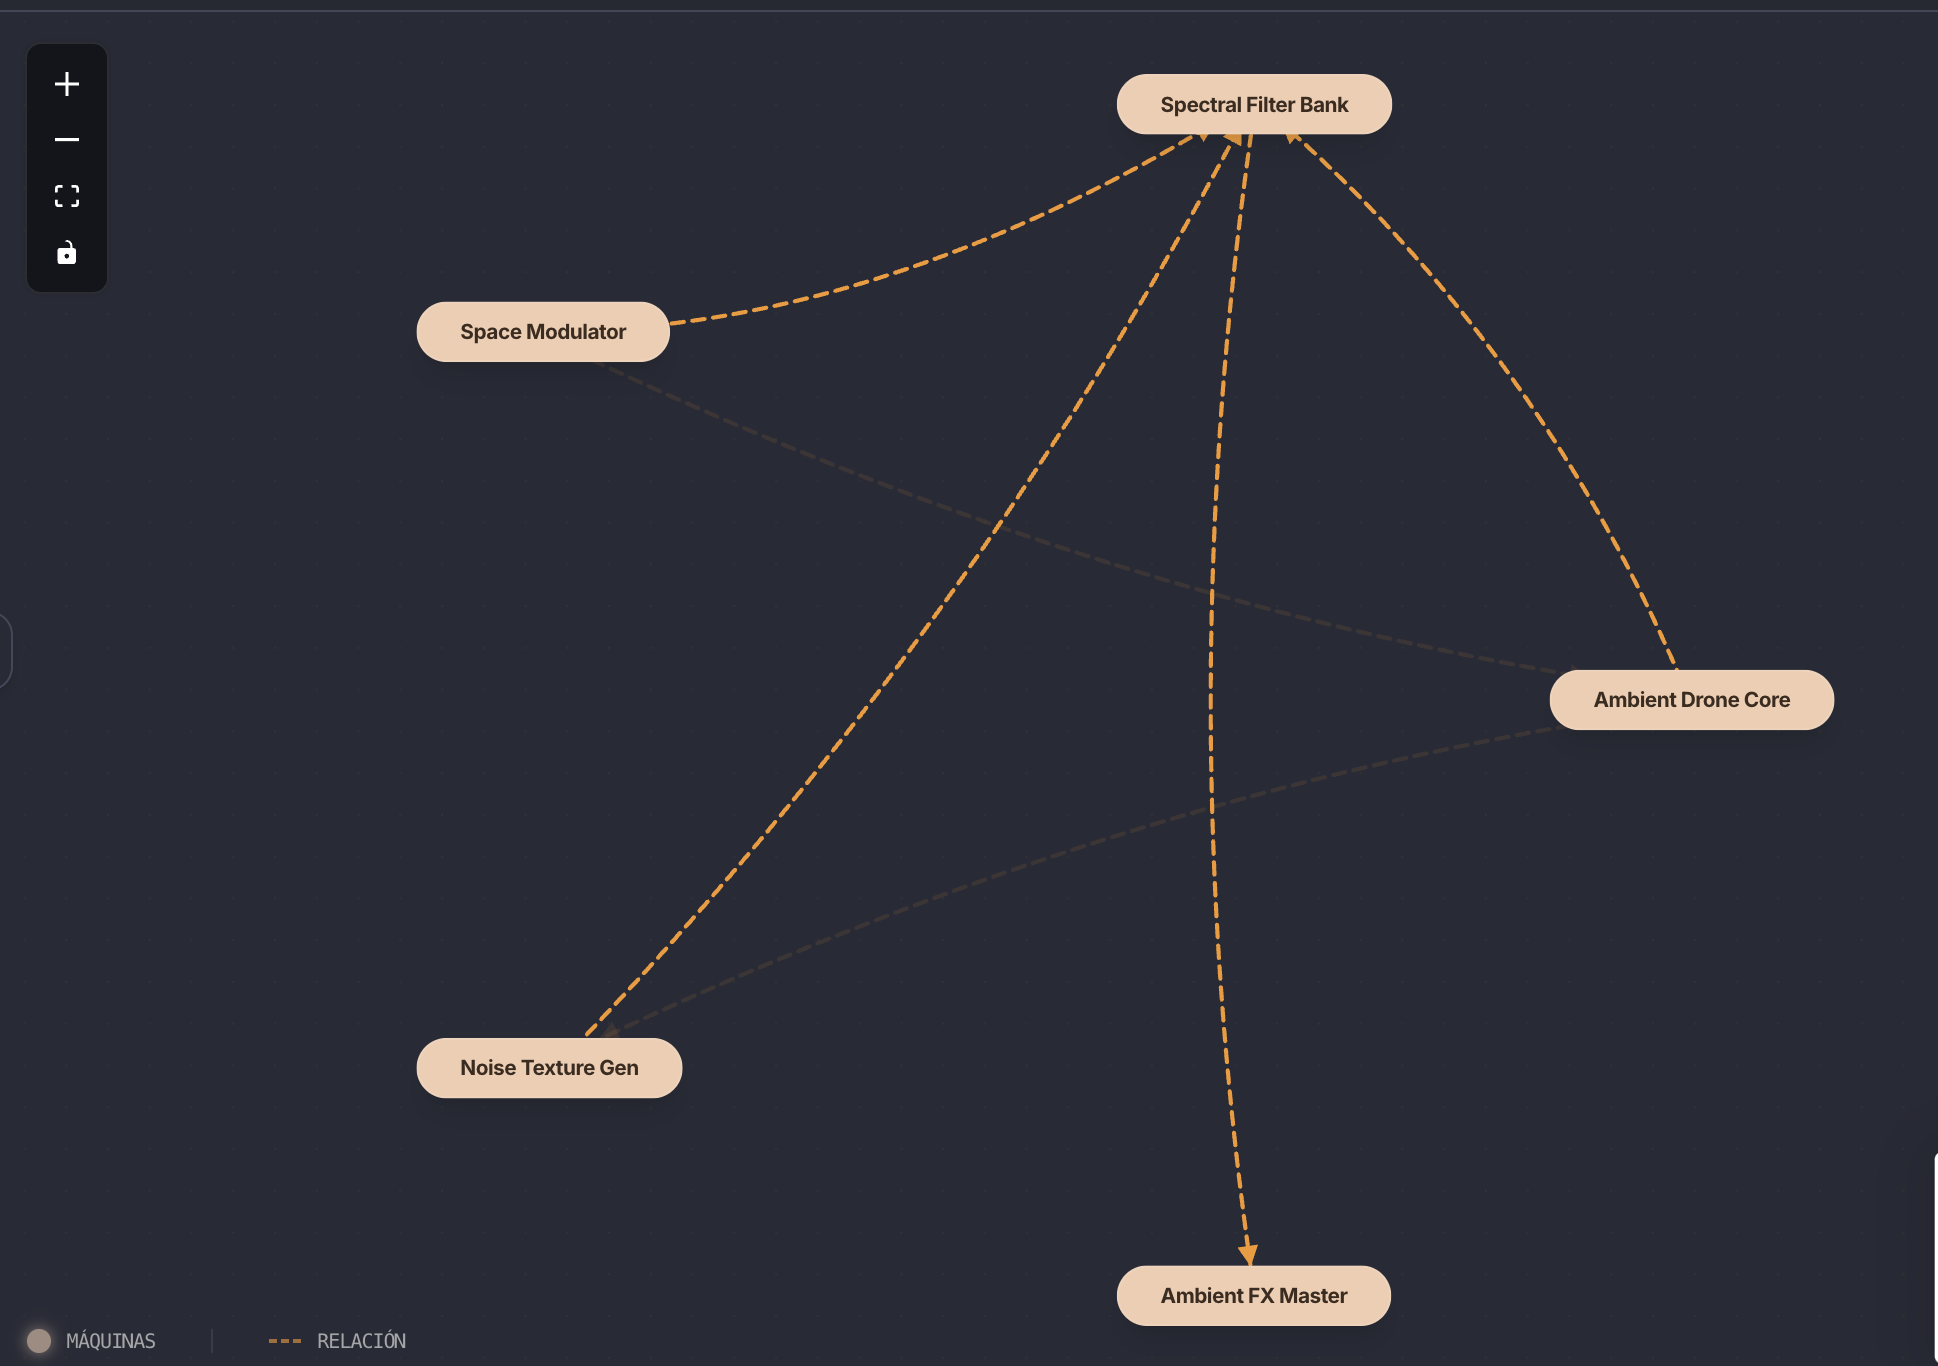
\includegraphics[width=\textwidth]{imagenes/05_analisis/09_nodoGrafoPulsado.png}
    \caption{Inspección de metadatos al seleccionar una máquina (nodo).}
\end{figure}

La interfaz es plenamente interactiva. Al pulsar sobre cualquier componente topológico (nodo o arista), se revela un panel de información detallada, permitiendo al usuario revisar la arquitectura sin analizar directamente el código subyacente.

\subsection{Editores de Relaciones}

\begin{figure}[!ht]
    \centering
    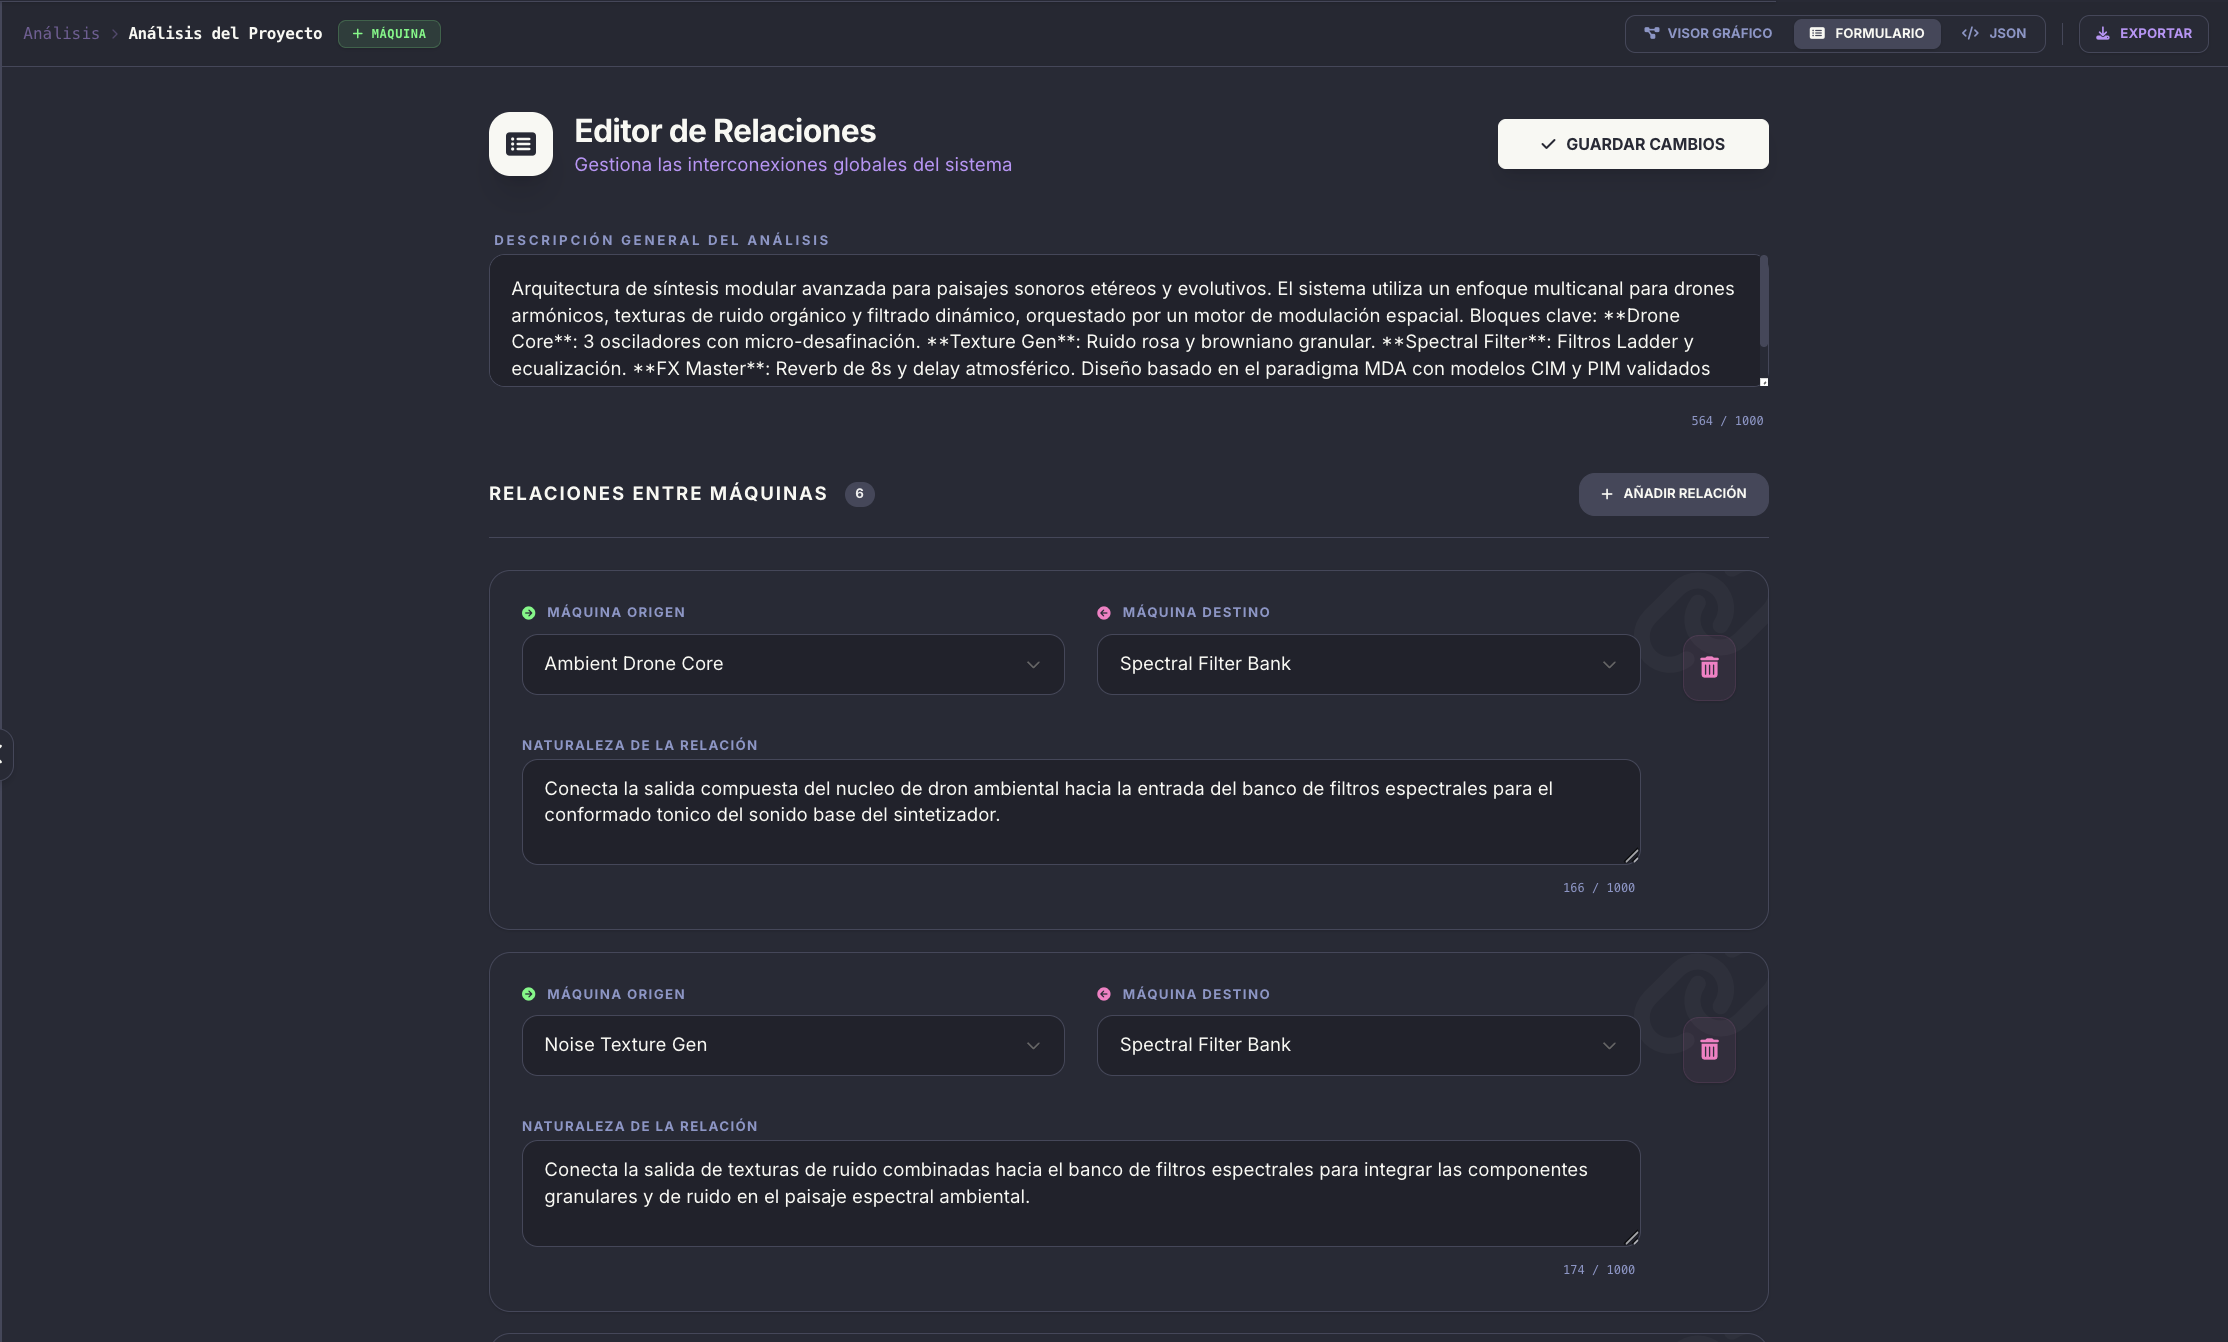
\includegraphics[width=\textwidth]{imagenes/05_analisis/10_editorFormularioRelacionesCim.png}
    \caption{Editor de relaciones mediante interfaz de formulario.}
\end{figure}

Para una edición asistida y visual, el editor de formularios posibilita la creación y alteración de enlaces seleccionando orígenes y destinos a través de selectores amigables.

\begin{figure}[!ht]
    \centering
    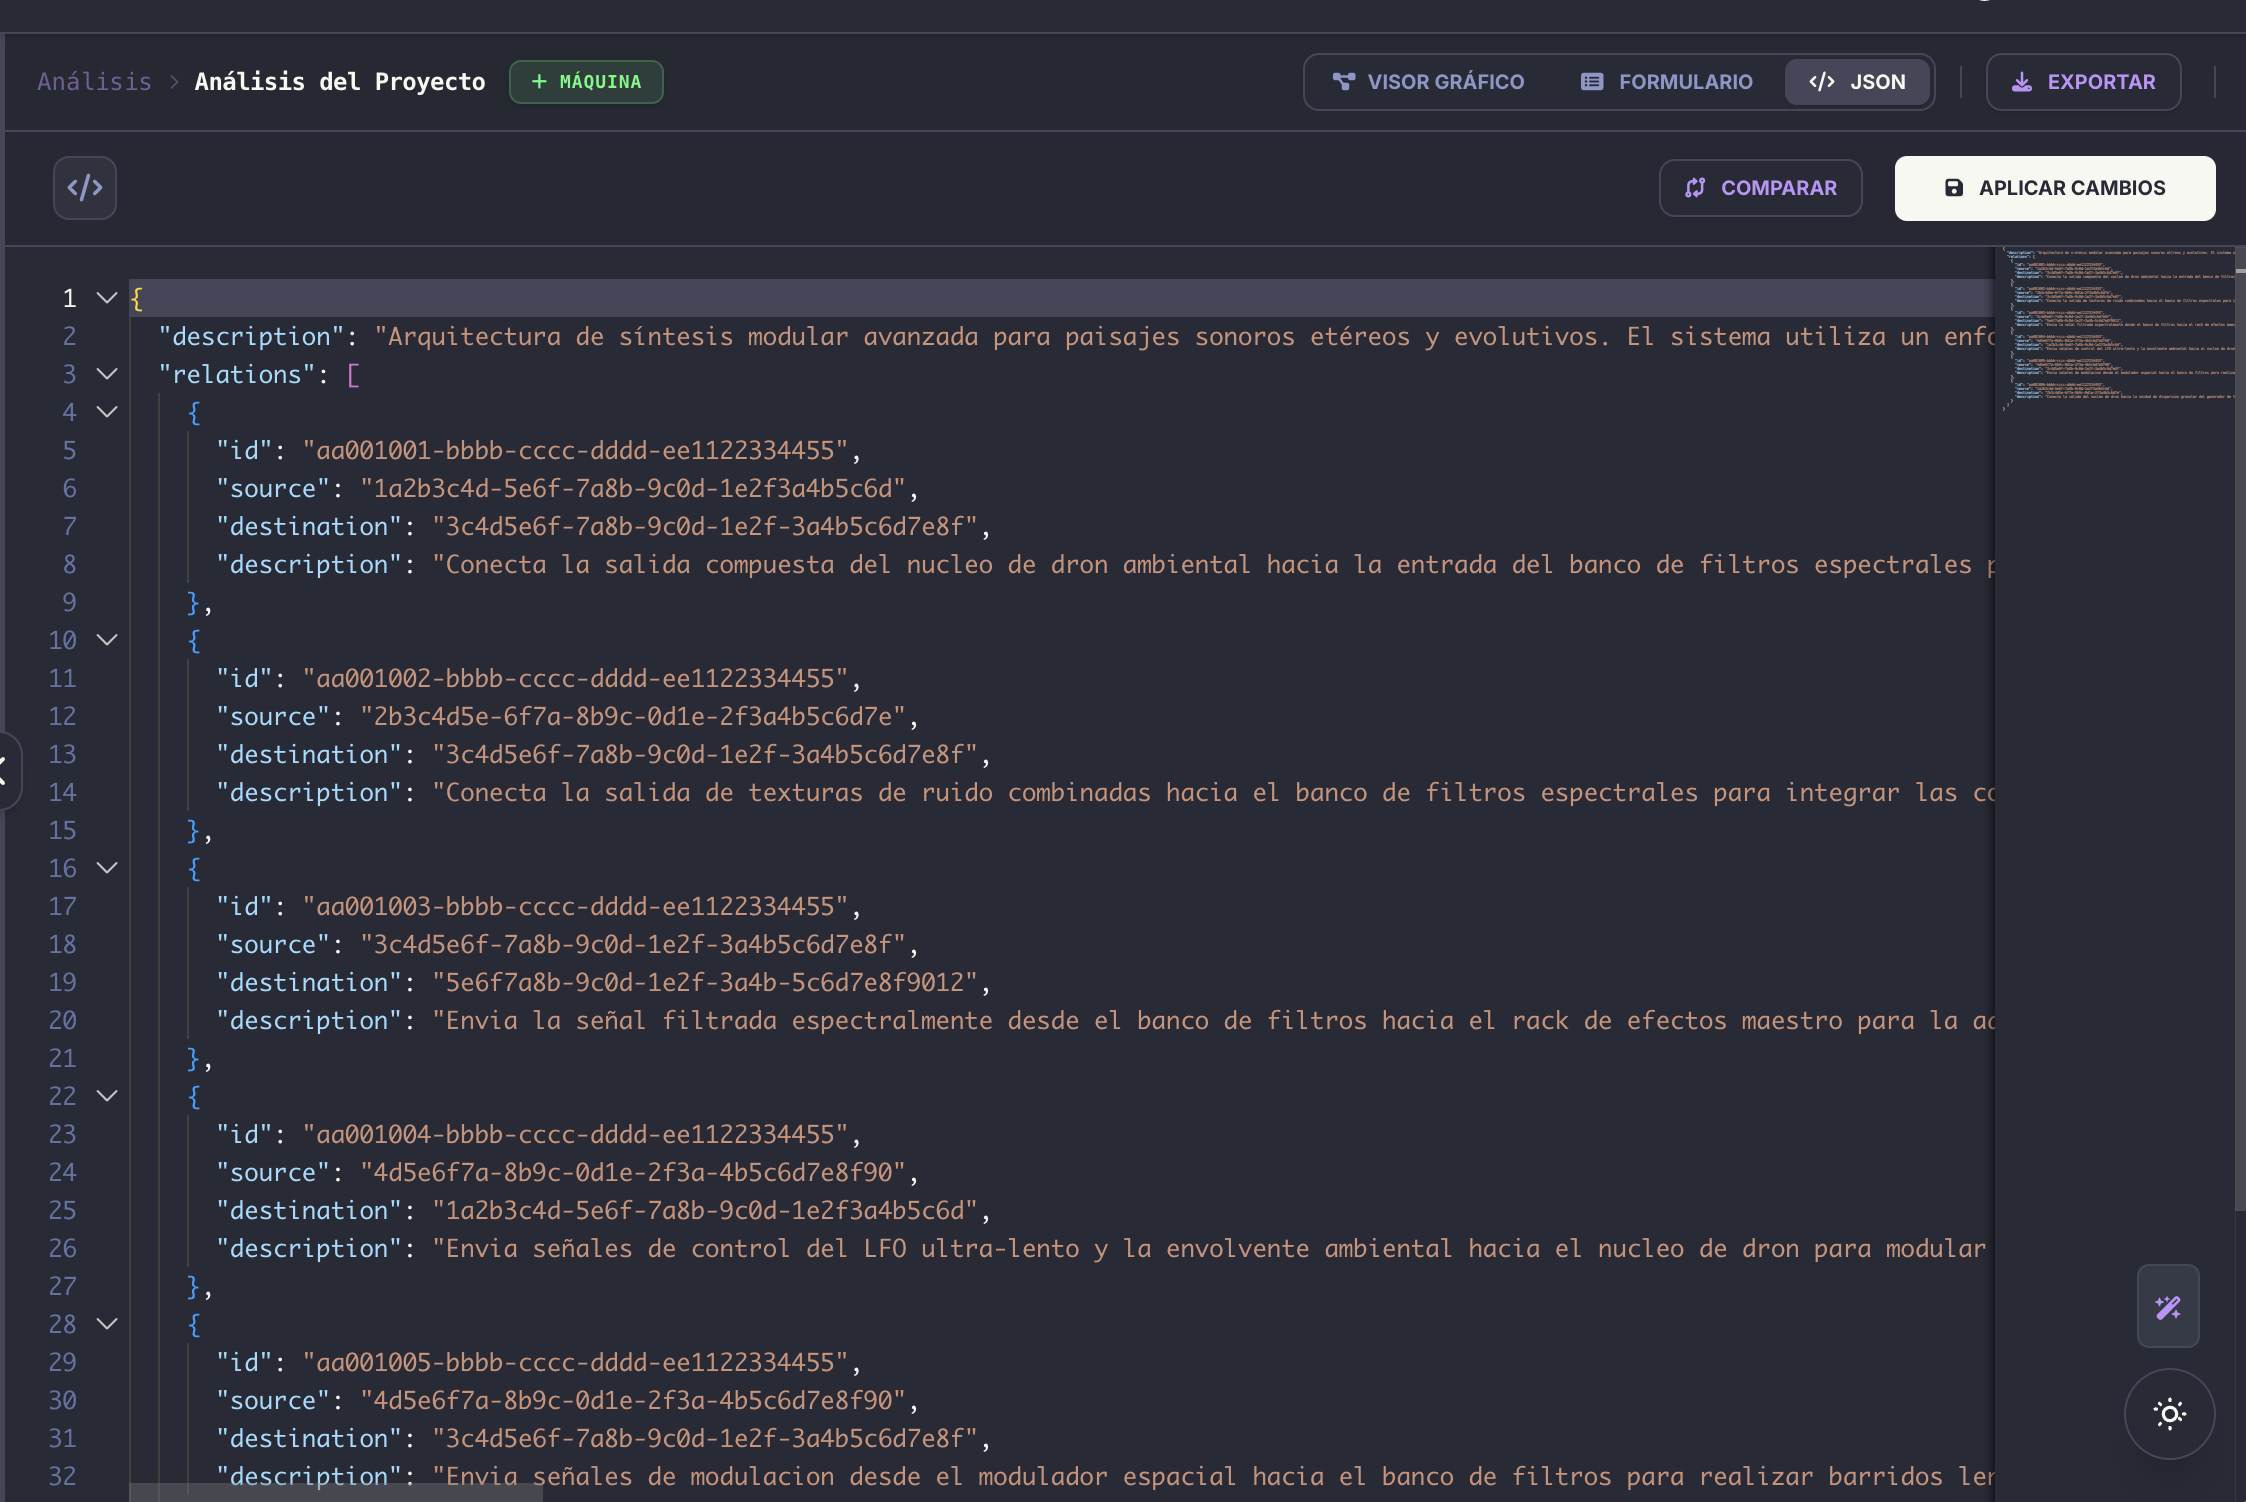
\includegraphics[width=\textwidth]{imagenes/05_analisis/11_edicionJsonRelacionesCim.png}
    \caption{Editor avanzado de código fuente (JSON) para las relaciones CIM.}
\end{figure}

Los usuarios familiarizados con la especificación \textit{DSL} pueden trabajar directamente sobre el código \textit{JSON}. Este editor incluye autocompletado y resaltado sintáctico.

\begin{figure}[!ht]
    \centering
    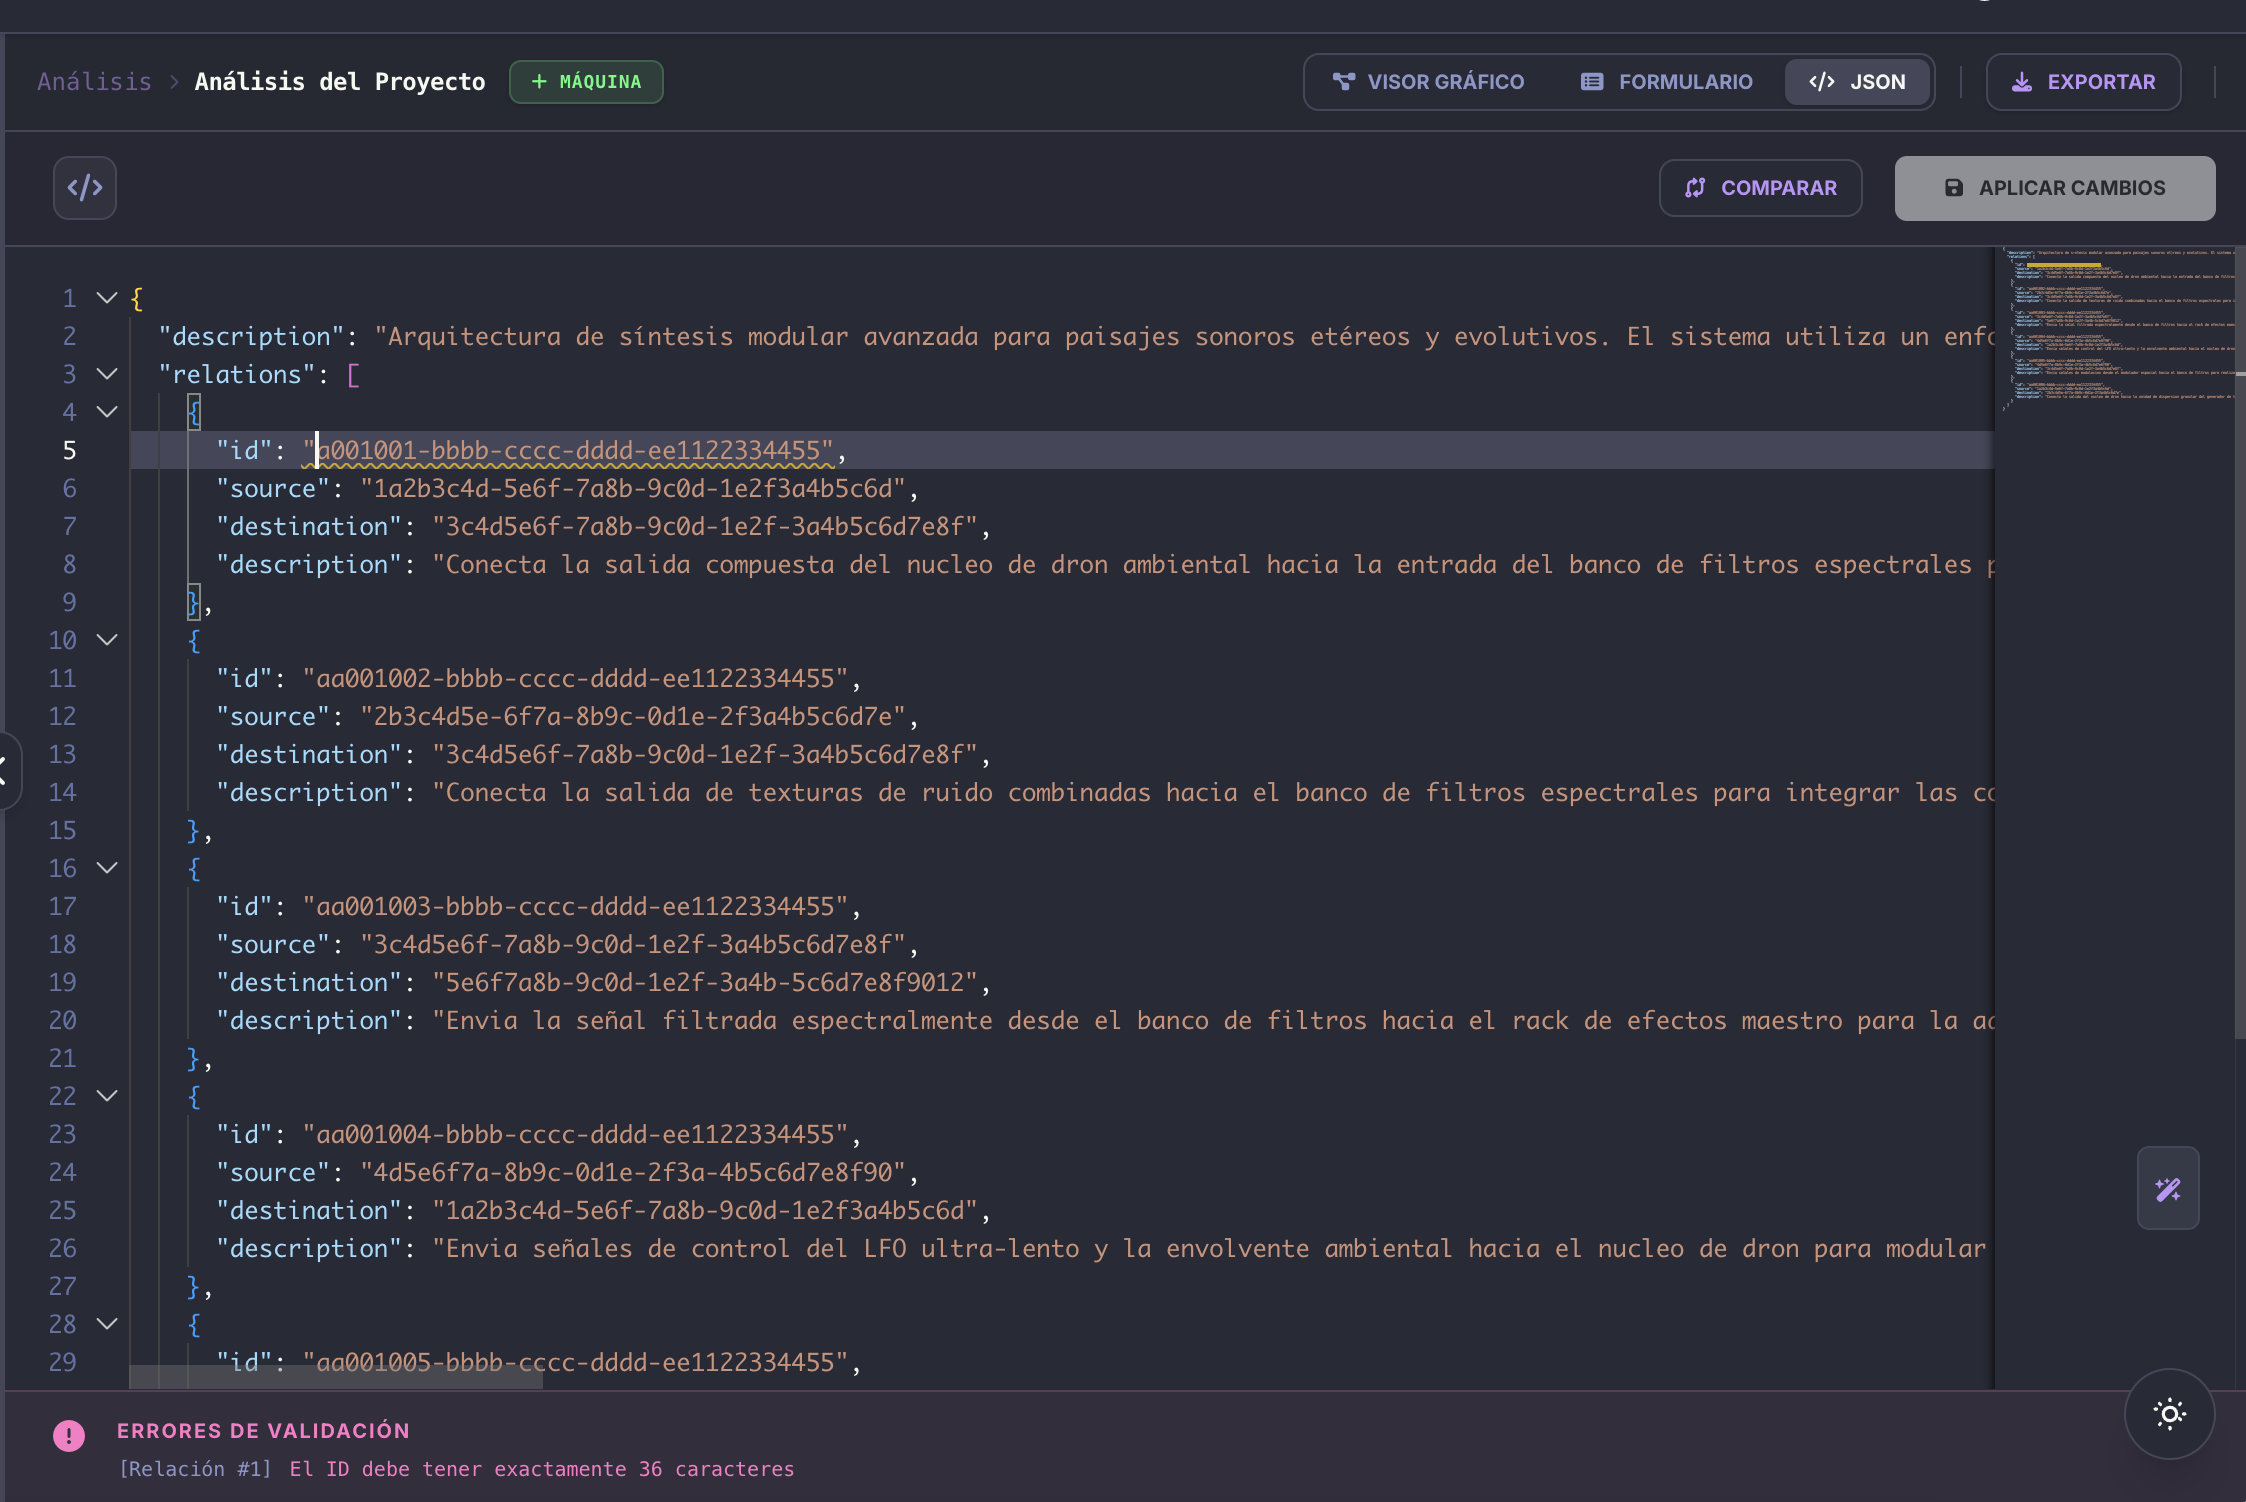
\includegraphics[width=\textwidth]{imagenes/05_analisis/12_gestionErroresEditorJsonRelacionesCim.png}
    \caption{Sistema de validación en tiempo real en el editor JSON.}
\end{figure}

El sistema verifica la estructura de forma continua. Ante un defecto sintáctico o un incumplimiento del modelo de dominio, el editor señala el error explícitamente, bloqueando el guardado de modelos inconsistentes.

\begin{figure}[!ht]
    \centering
    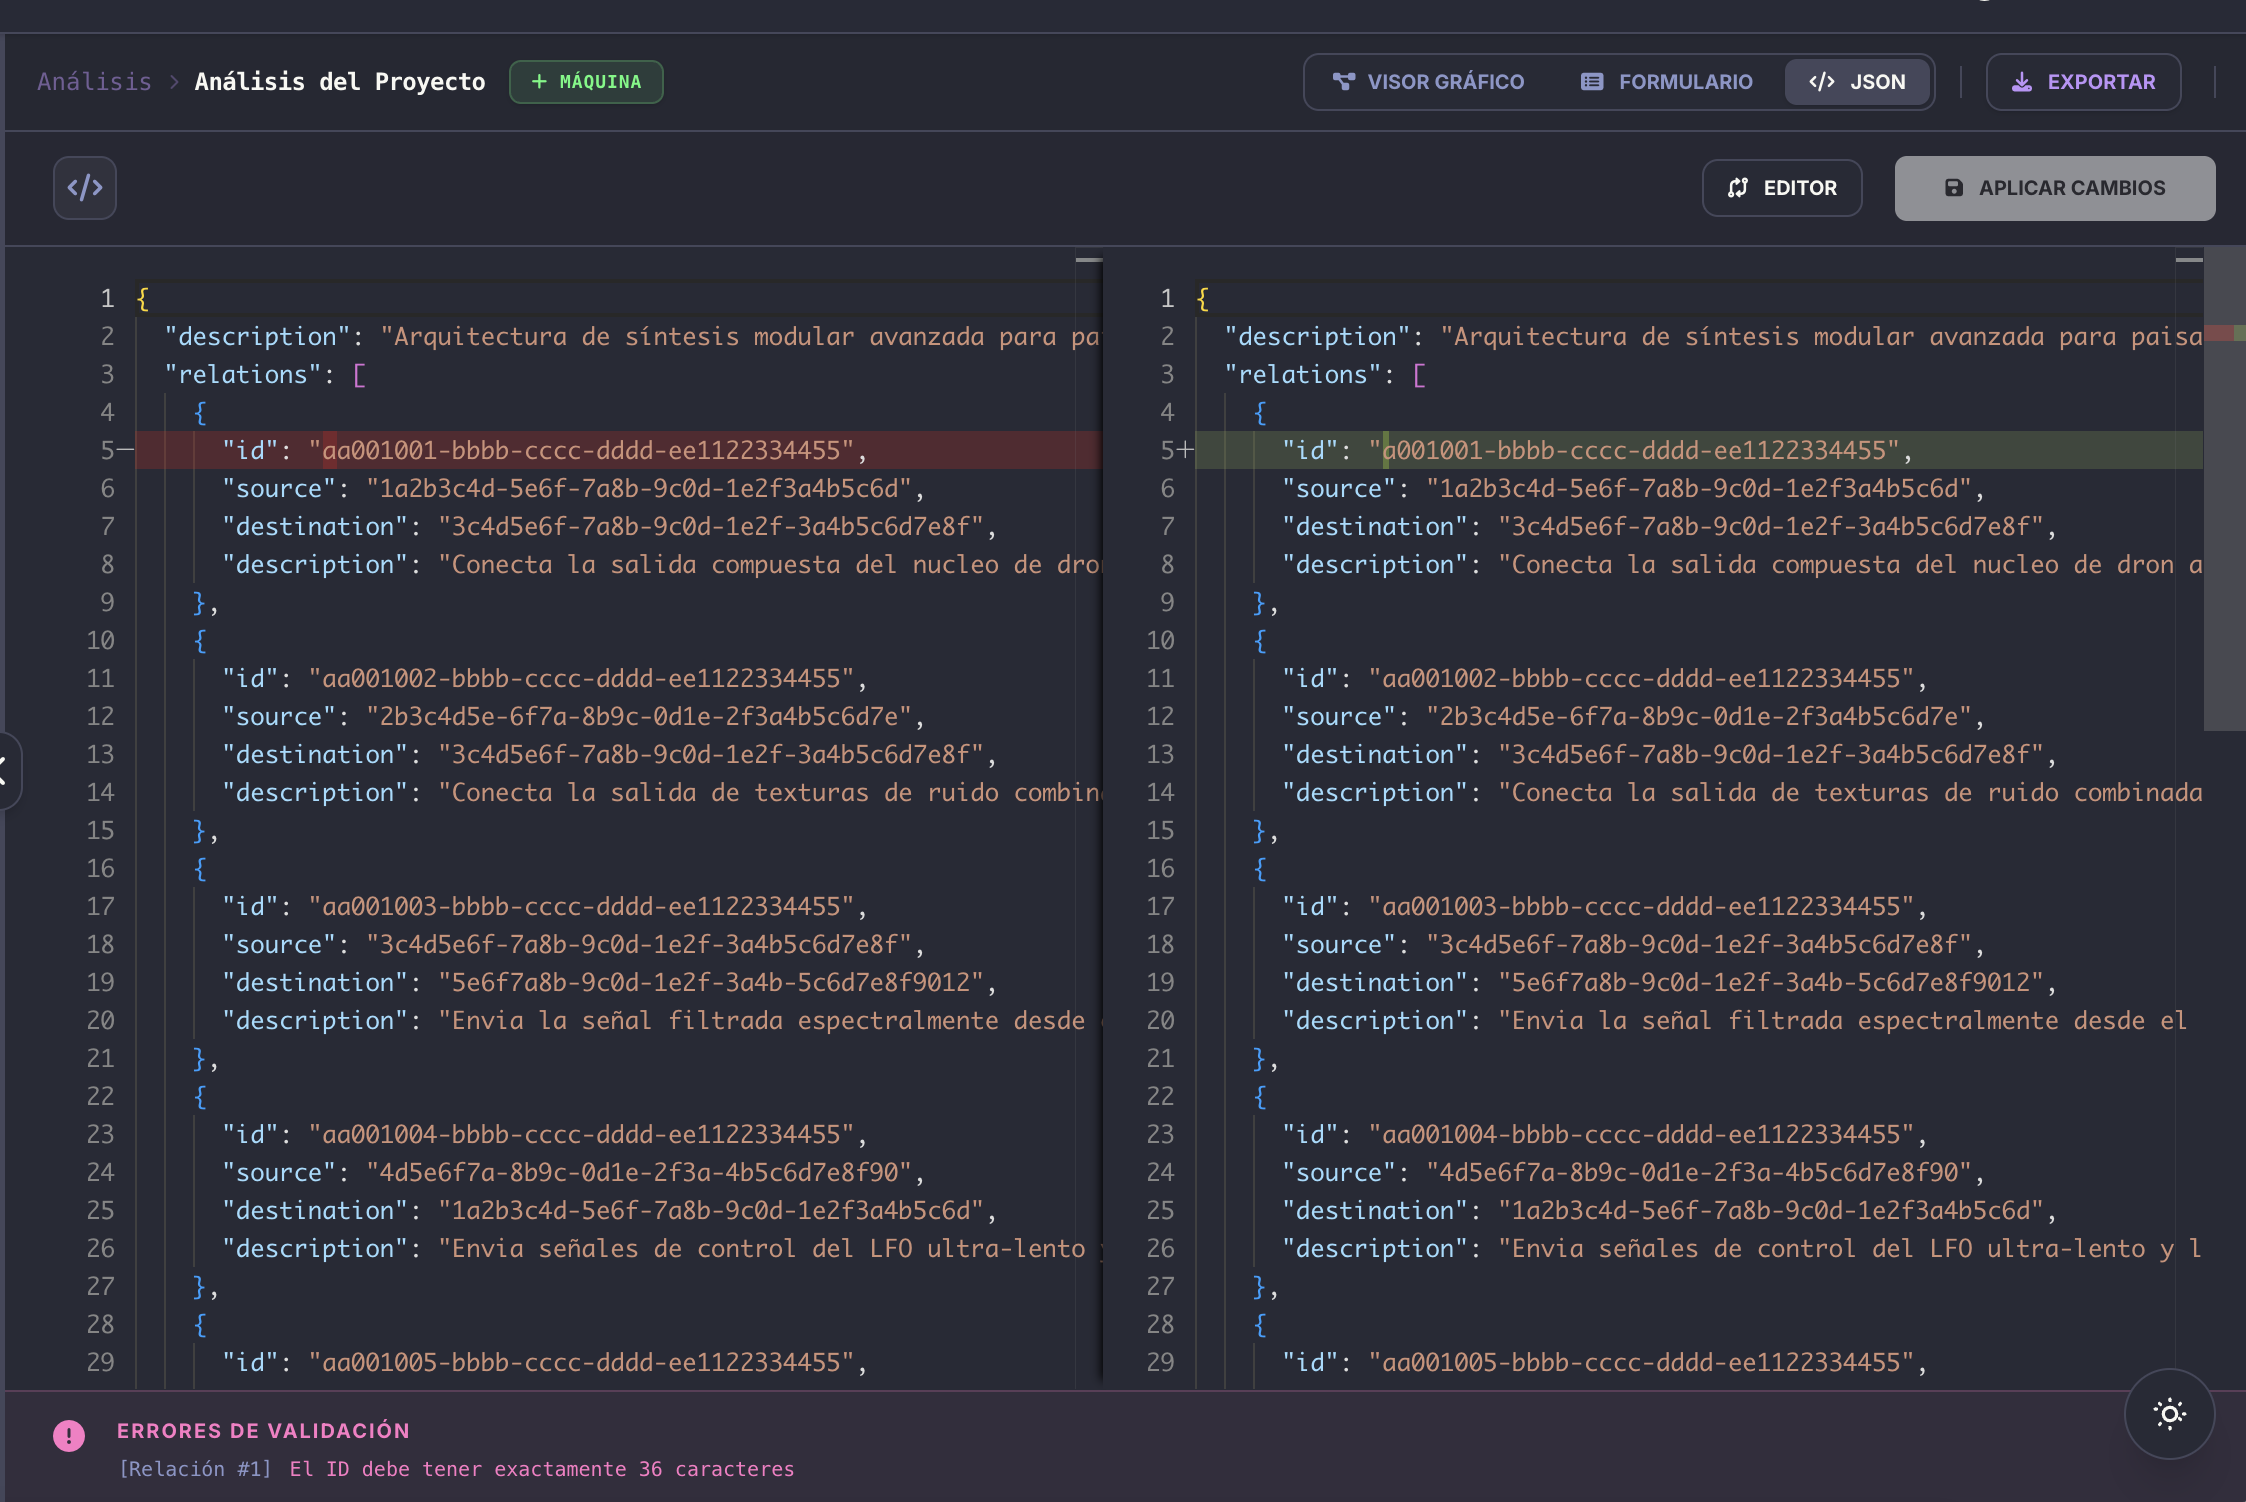
\includegraphics[width=\textwidth]{imagenes/05_analisis/13_comparadorEditorJsonRelacionesCim.png}
    \caption{Herramienta visual de diferencias (Diff) en el editor JSON.}
\end{figure}

Para gestionar cambios complejos, la herramienta de \textit{diff} permite comparar las alteraciones en curso con la última versión guardada, garantizando un control de versiones a nivel de sesión.

\begin{figure}[!ht]
    \centering
    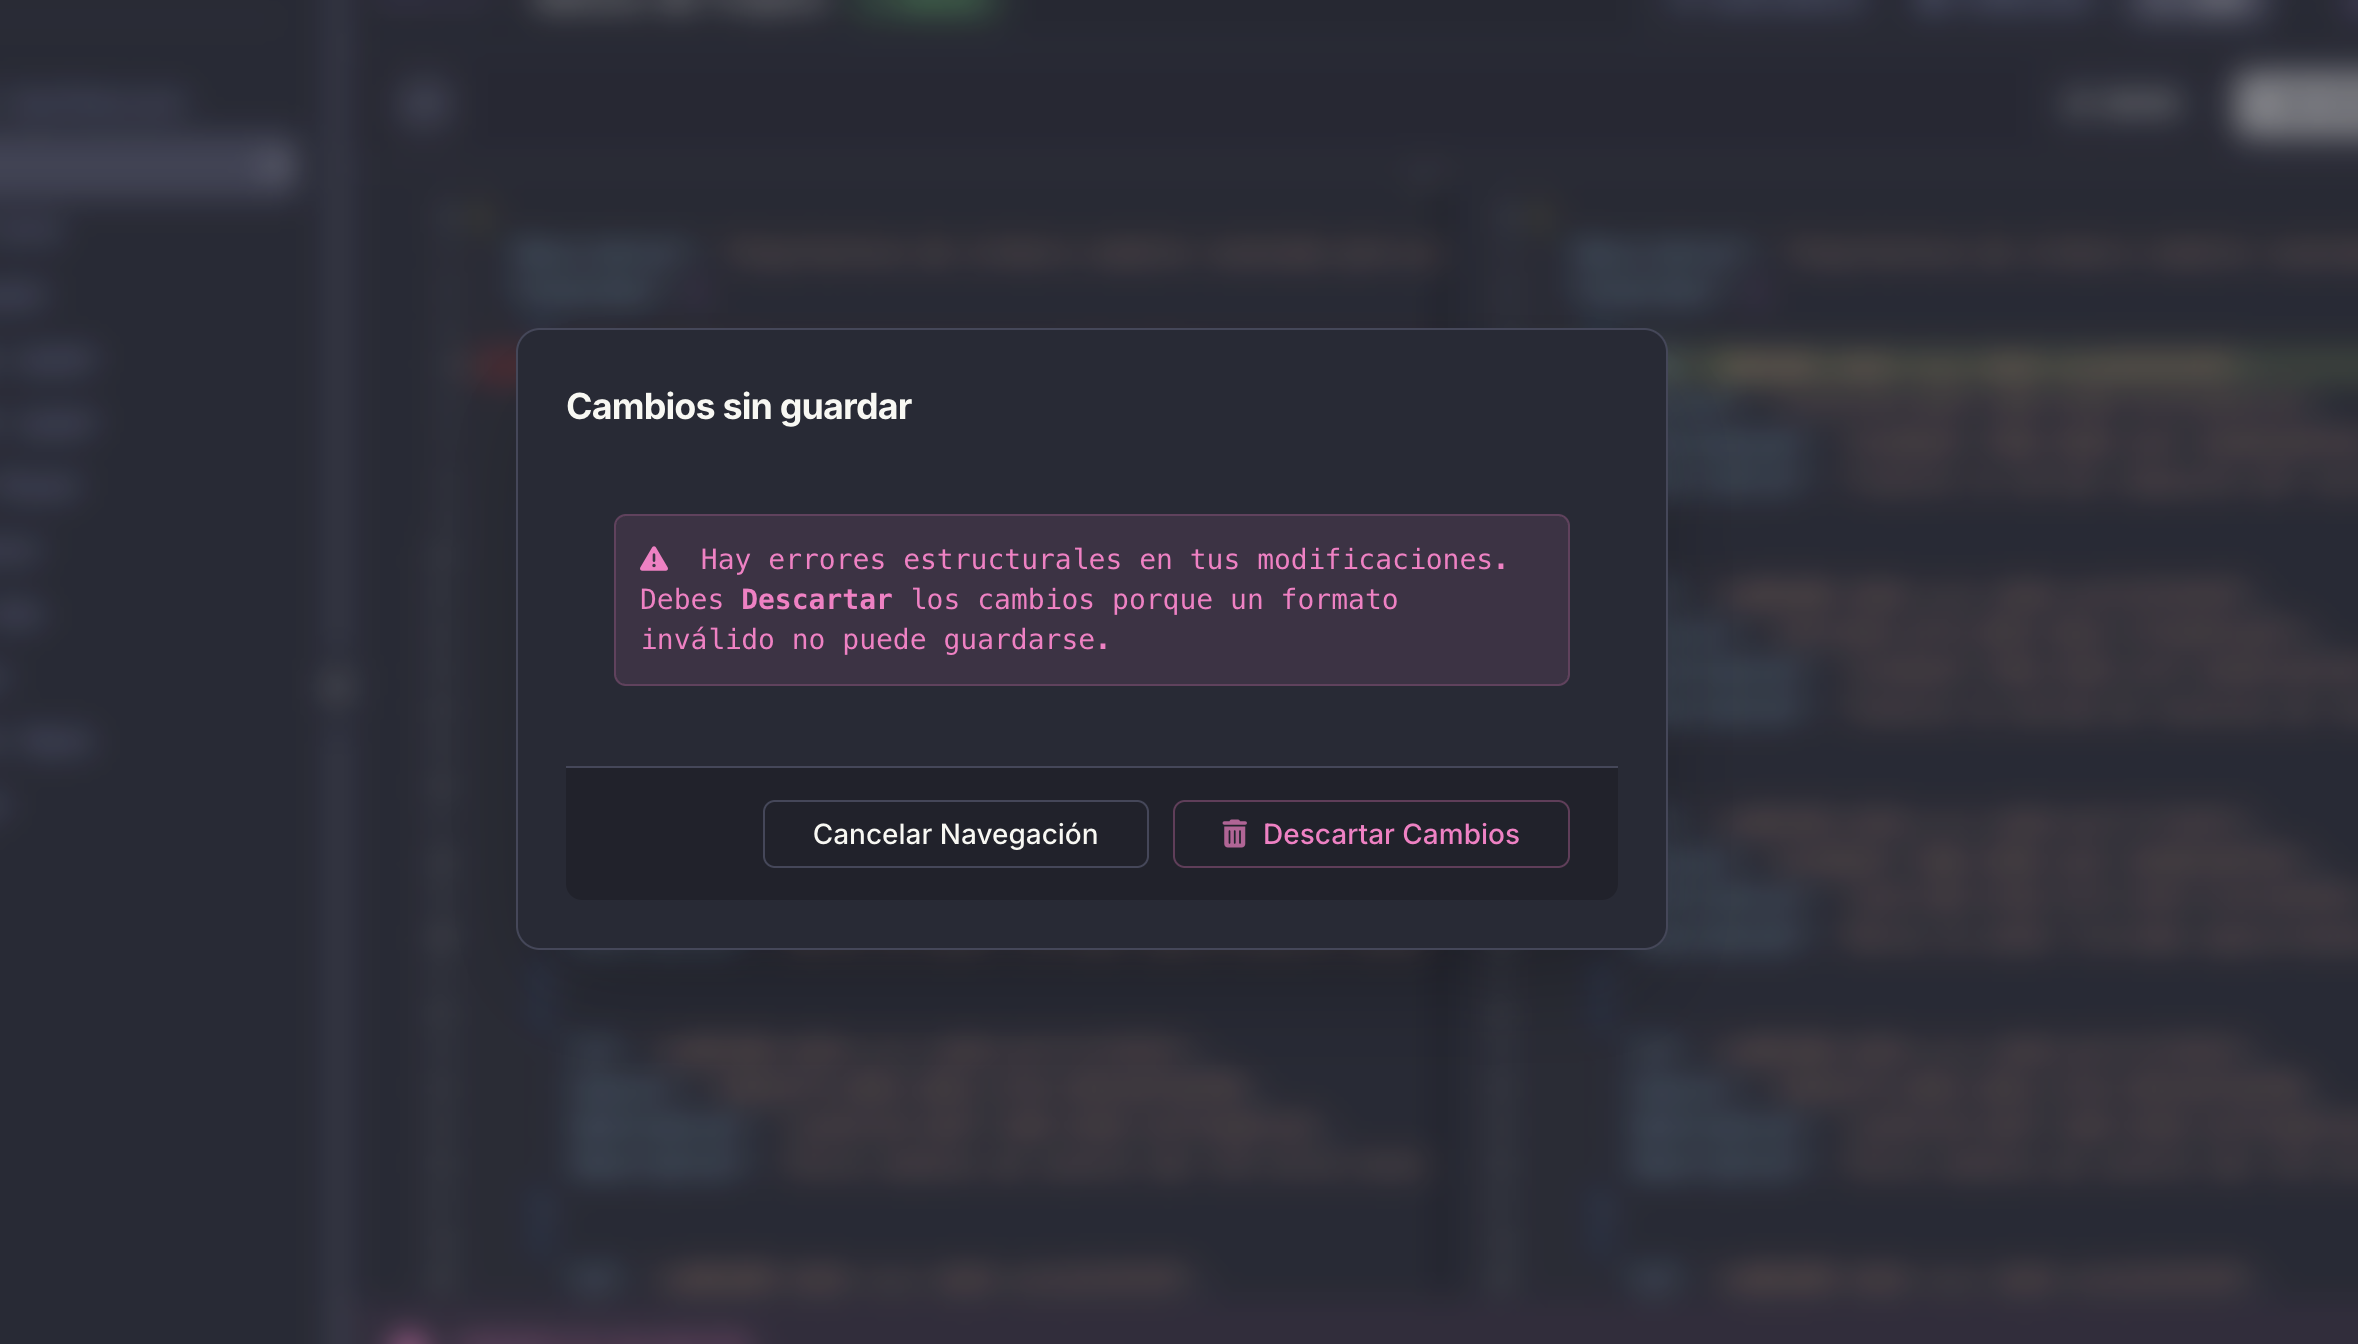
\includegraphics[width=0.6\textwidth]{imagenes/05_analisis/15_cambiarDePantallaSinGuardarJsonRelacionesCim.png}
    \caption{Aviso preventivo por cambios no guardados.}
\end{figure}

\begin{figure}[!ht]
    \centering
    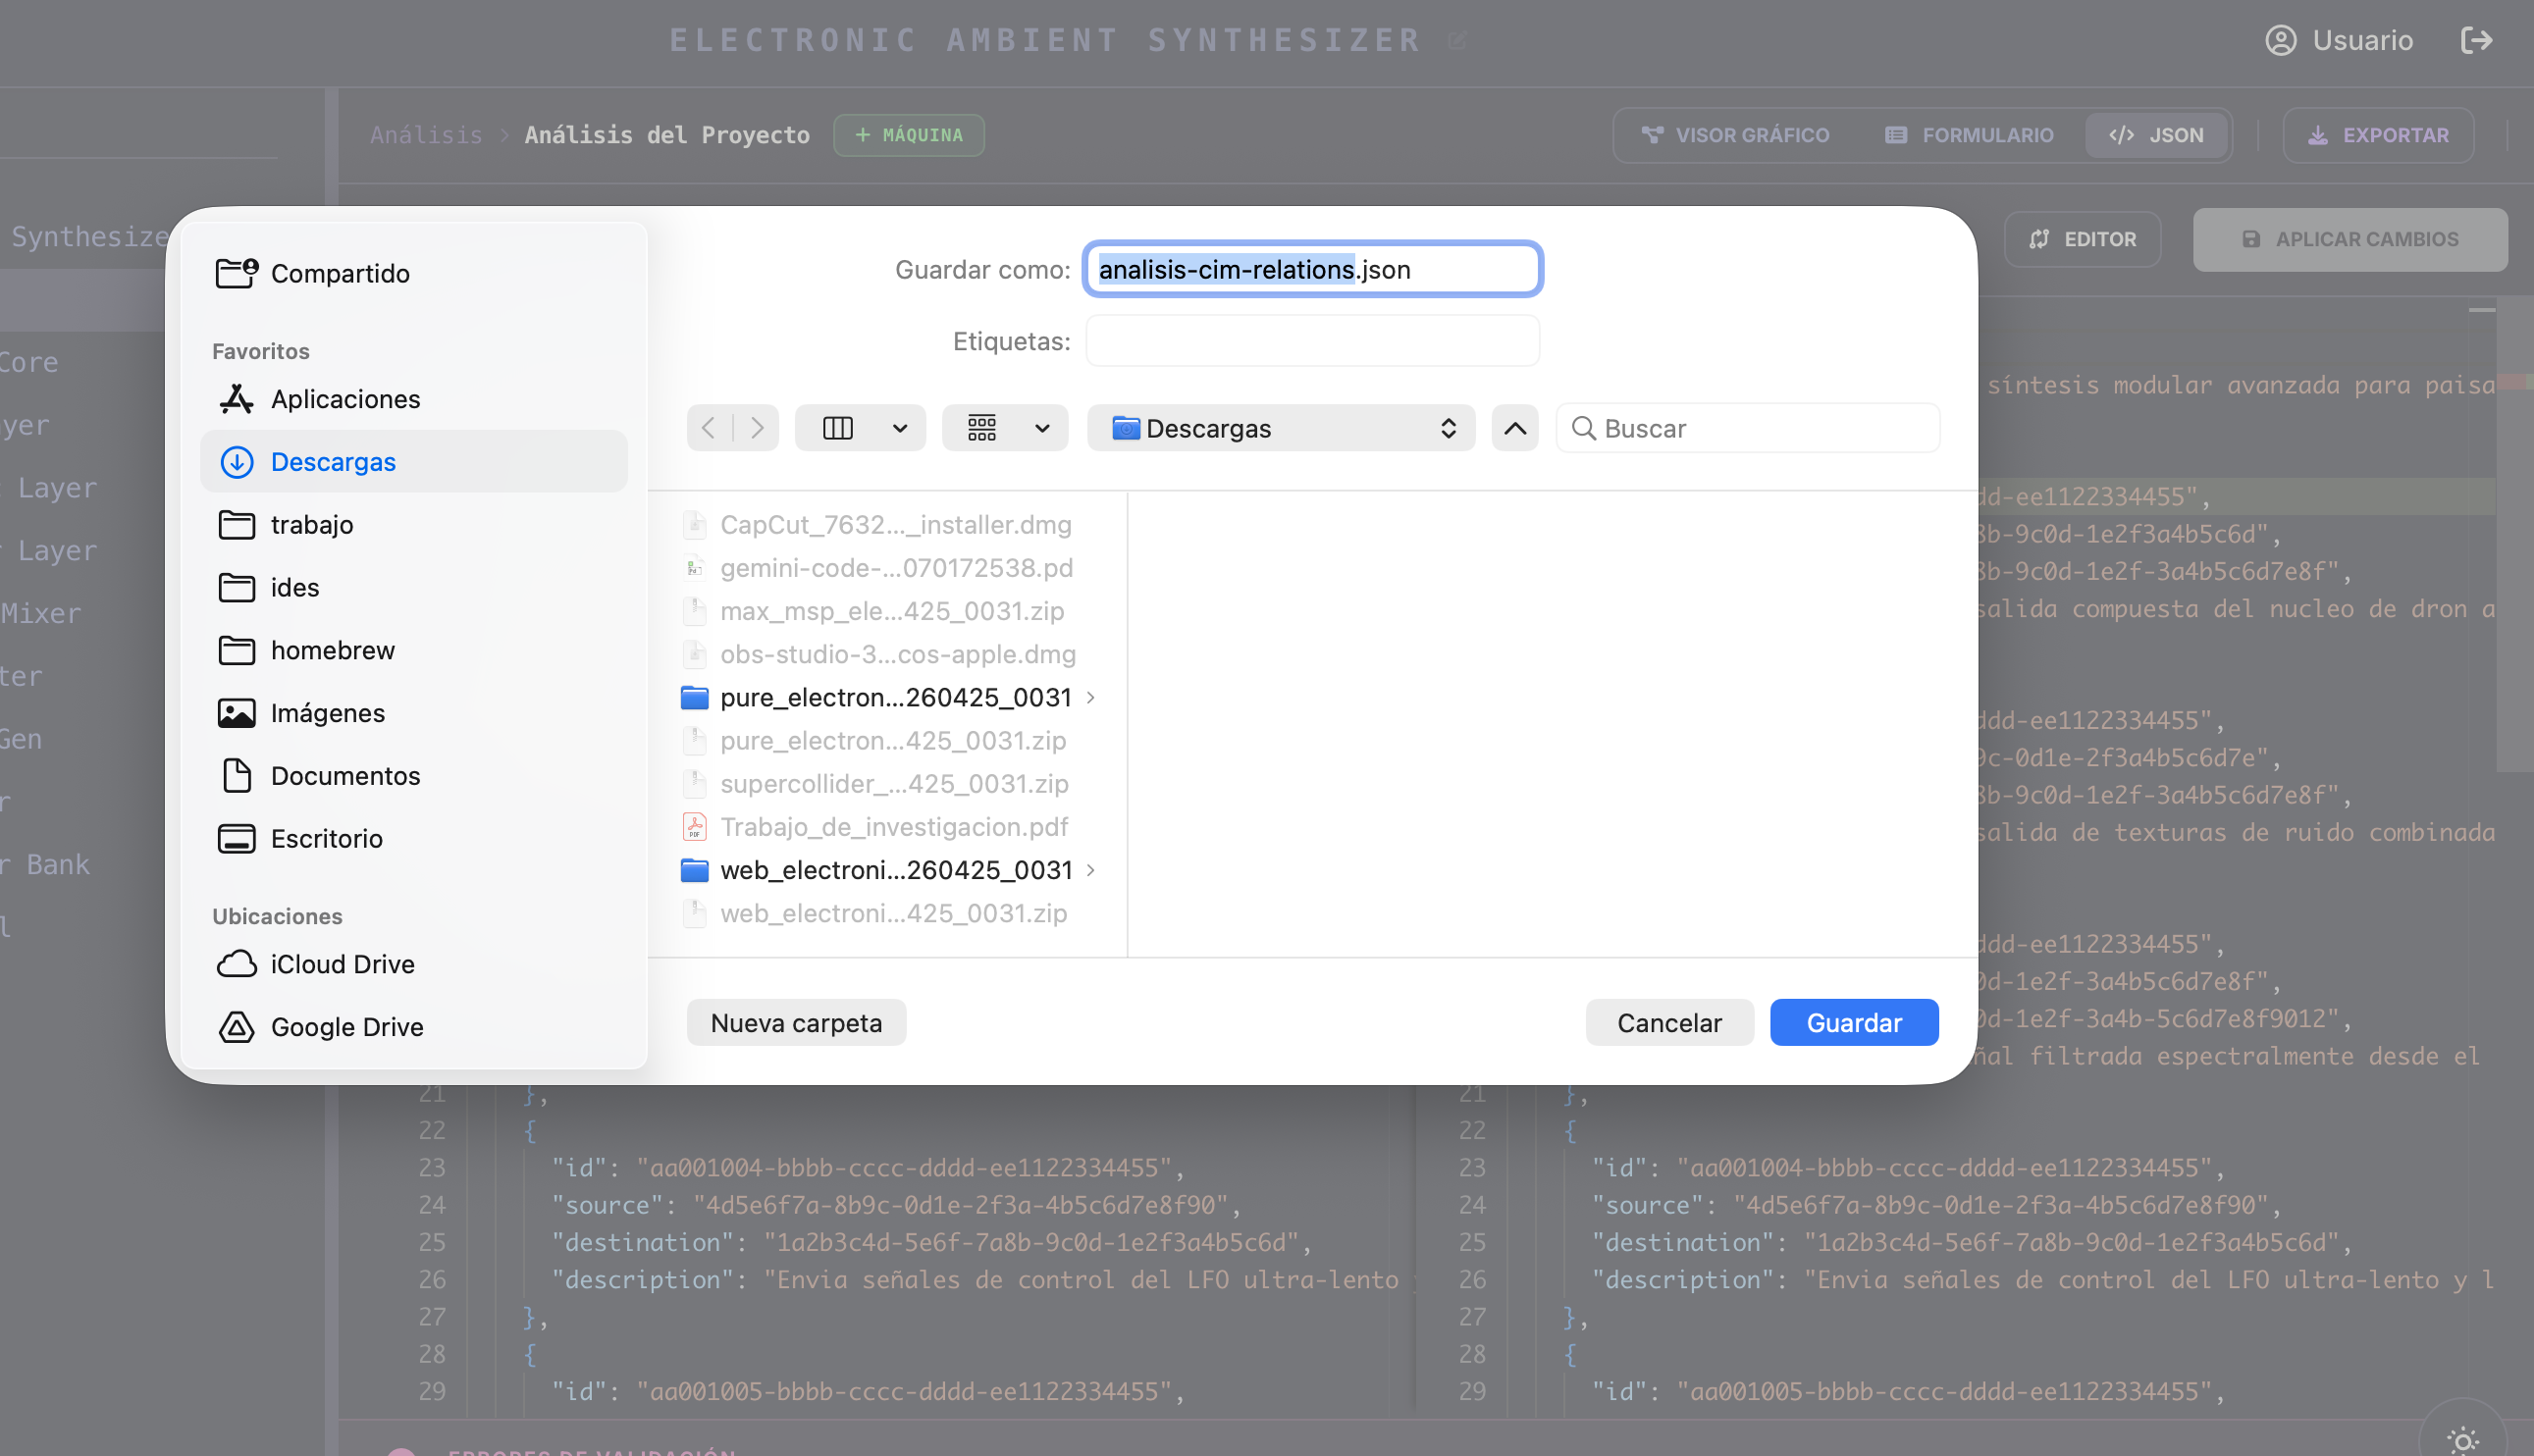
\includegraphics[width=0.6\textwidth]{imagenes/05_analisis/14_exportacionJsonRelacionesCim.png}
    \caption{Opciones de exportación del modelo de relaciones.}
\end{figure}

El entorno cuenta con barreras de seguridad, advirtiendo al usuario si intenta cambiar de vista sin guardar. Asimismo, incluye capacidades de exportación para guardar localmente el modelo \textit{JSON} consolidado.

\section{Edición de Máquinas CIM Internas}

Una vez definida la red general, cada máquina conceptual requiere la configuración pormenorizada de su lógica interna y componentes de interfaz.

\begin{figure}[!ht]
    \centering
    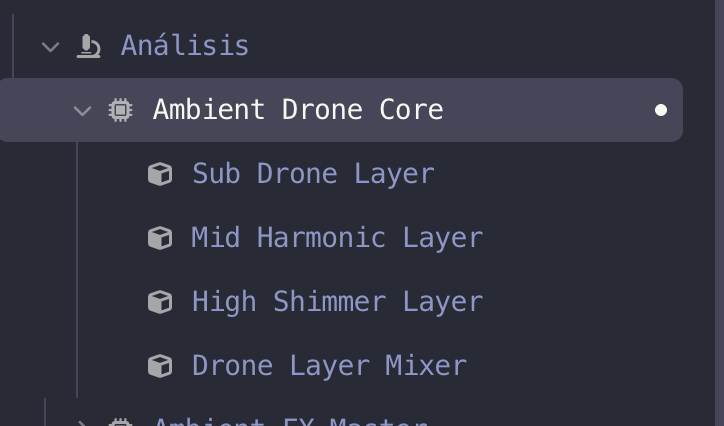
\includegraphics[width=0.4\textwidth]{imagenes/05_analisis/16_maquinaCimEnExplorador.png}
    \caption{Acceso a la configuración específica de una máquina CIM en el explorador.}
\end{figure}

Al seleccionar una máquina concreta en el árbol del explorador, se abre un panel focalizado en su arquitectura interna.

\begin{figure}[!ht]
    \centering
    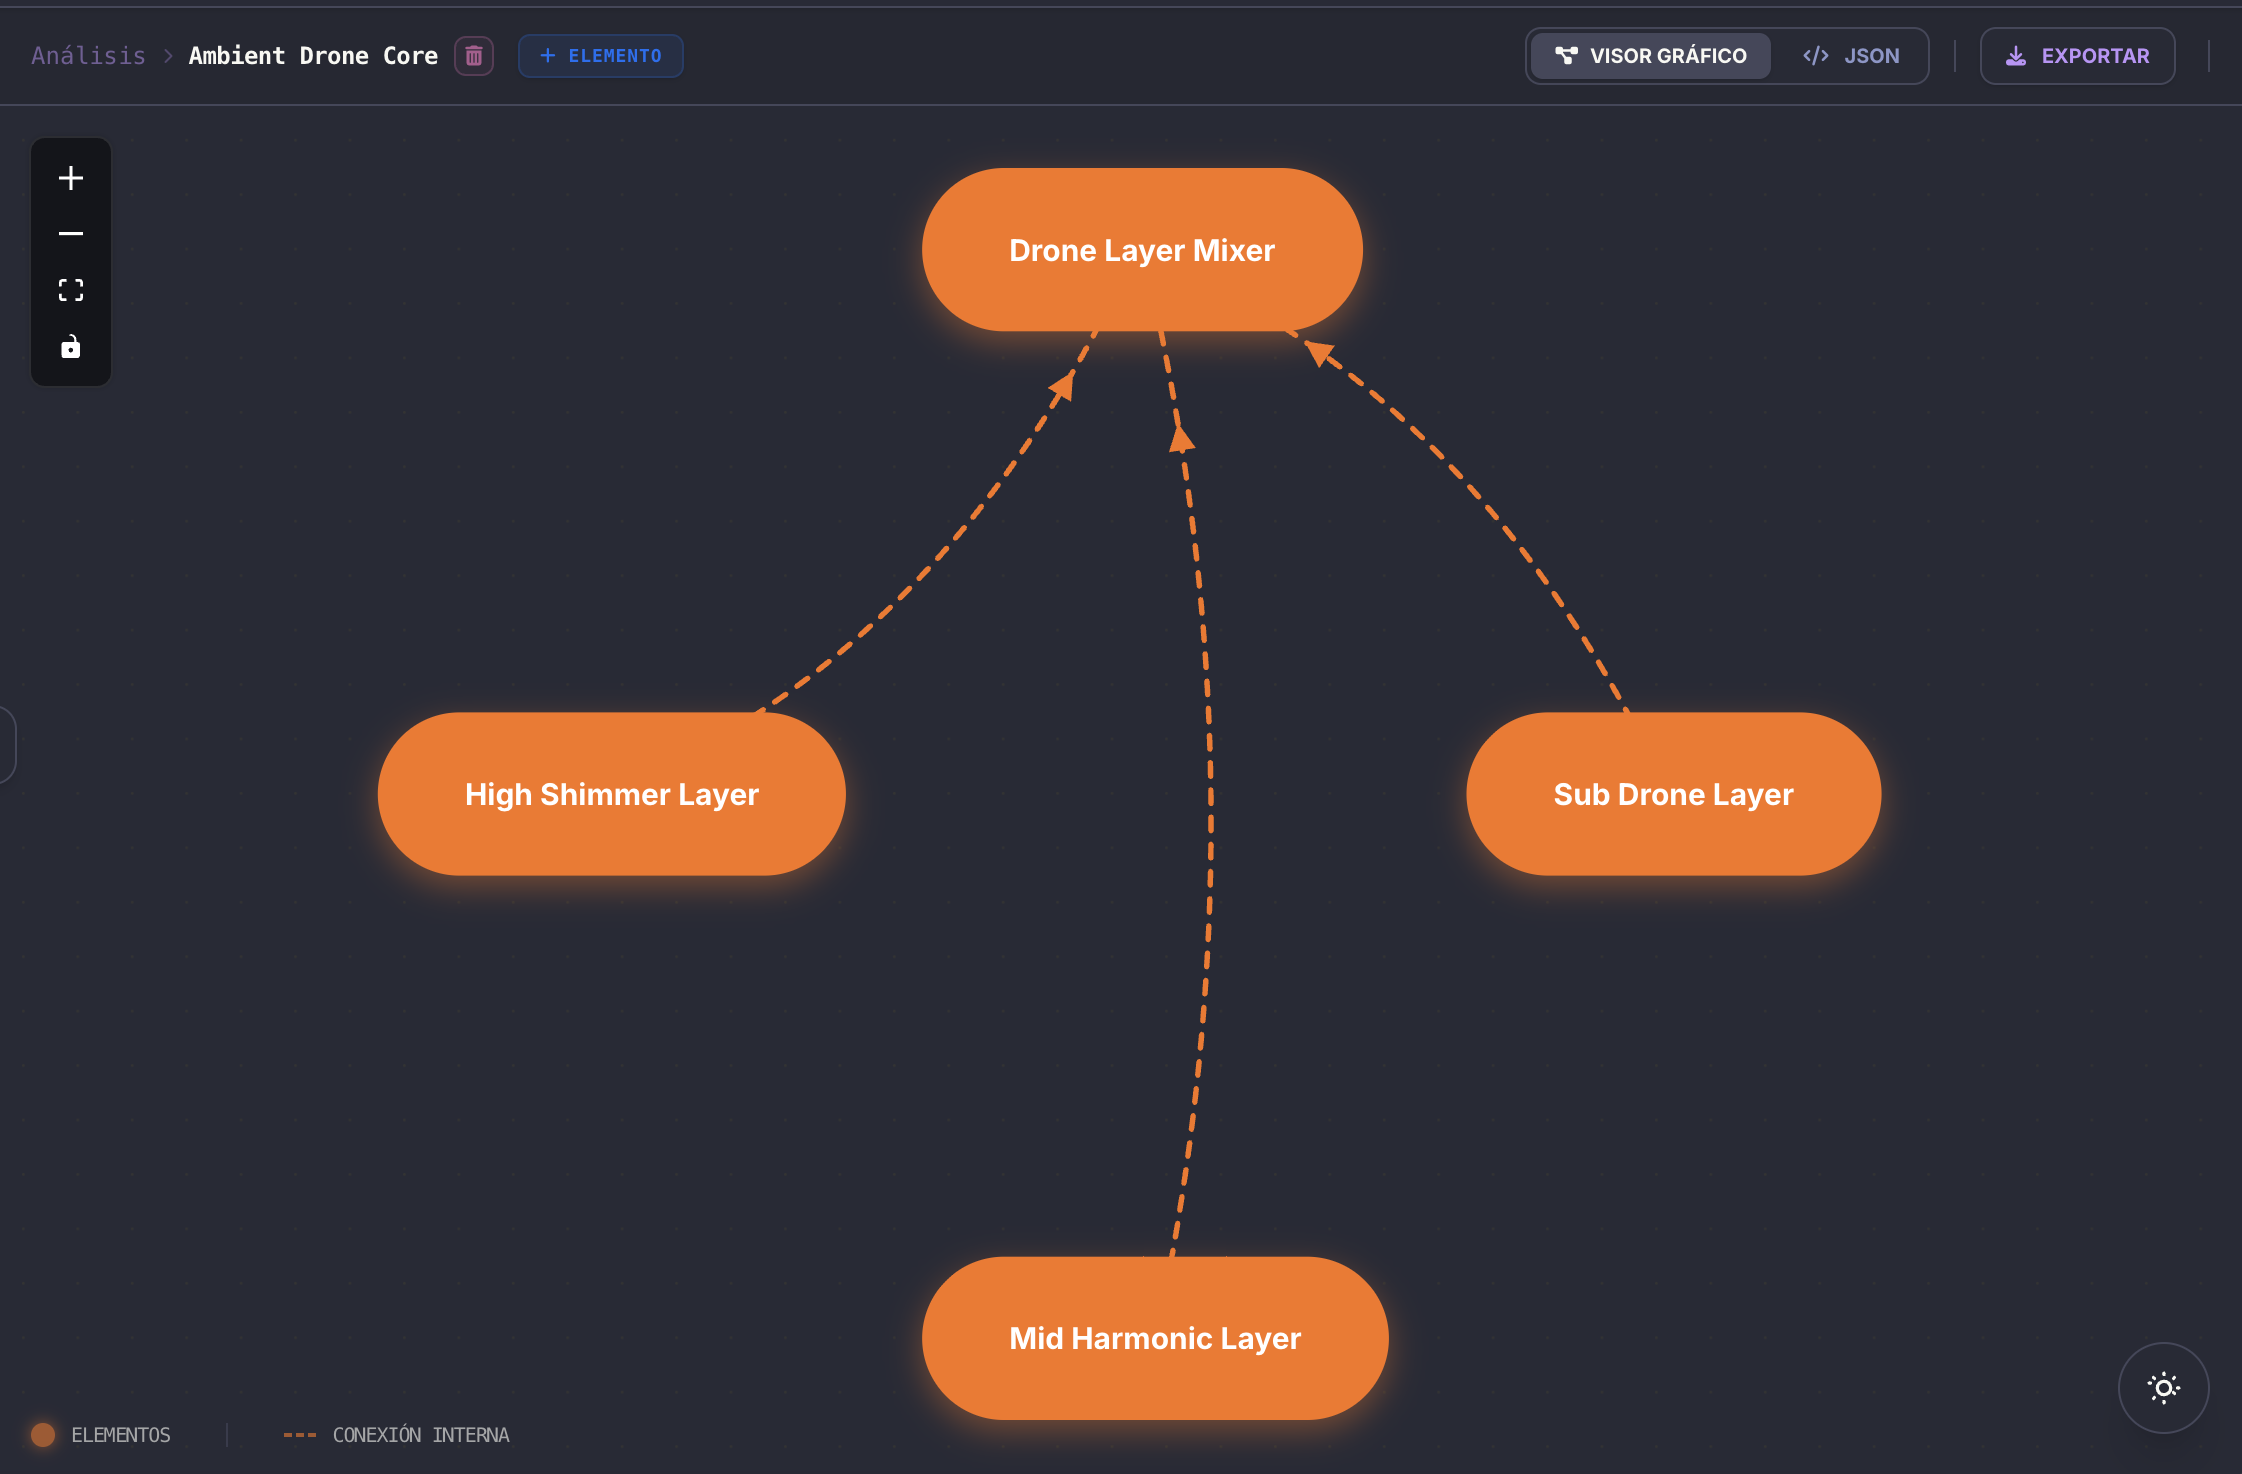
\includegraphics[width=\textwidth]{imagenes/05_analisis/17_visorGraficoMaquinaCim.png}
    \caption{Visor gráfico de la estructura interna de la máquina CIM.}
\end{figure}

\begin{figure}[!ht]
    \centering
    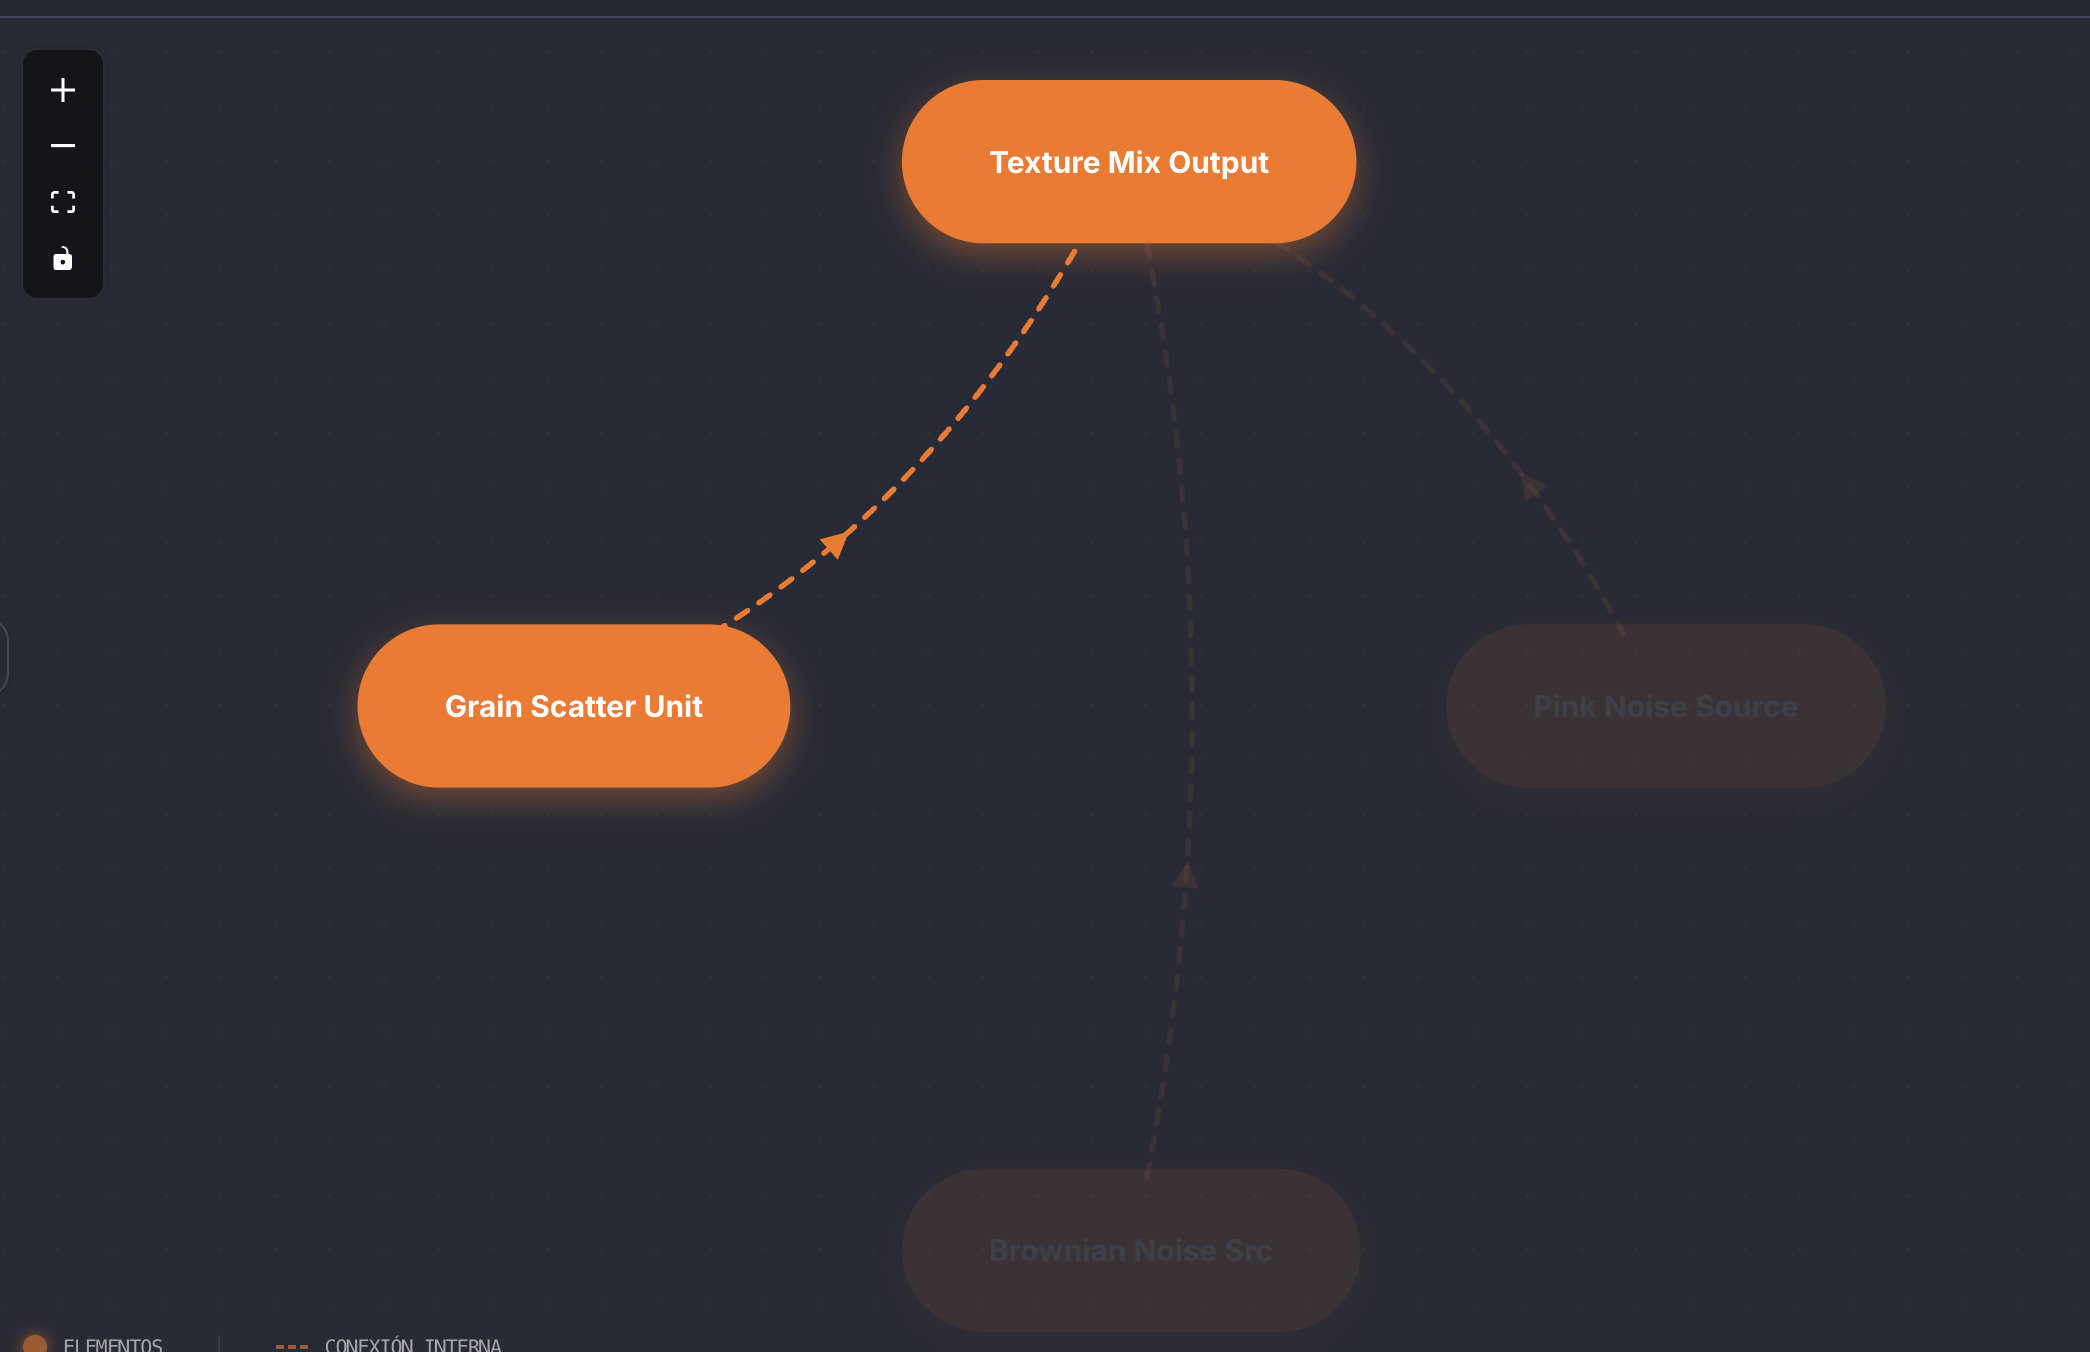
\includegraphics[width=\textwidth]{imagenes/05_analisis/18_visorGraficoMaquinaCimAristaPulsada.png}
    \caption{Inspección de las conexiones lógicas internas.}
\end{figure}

\begin{figure}[!ht]
    \centering
    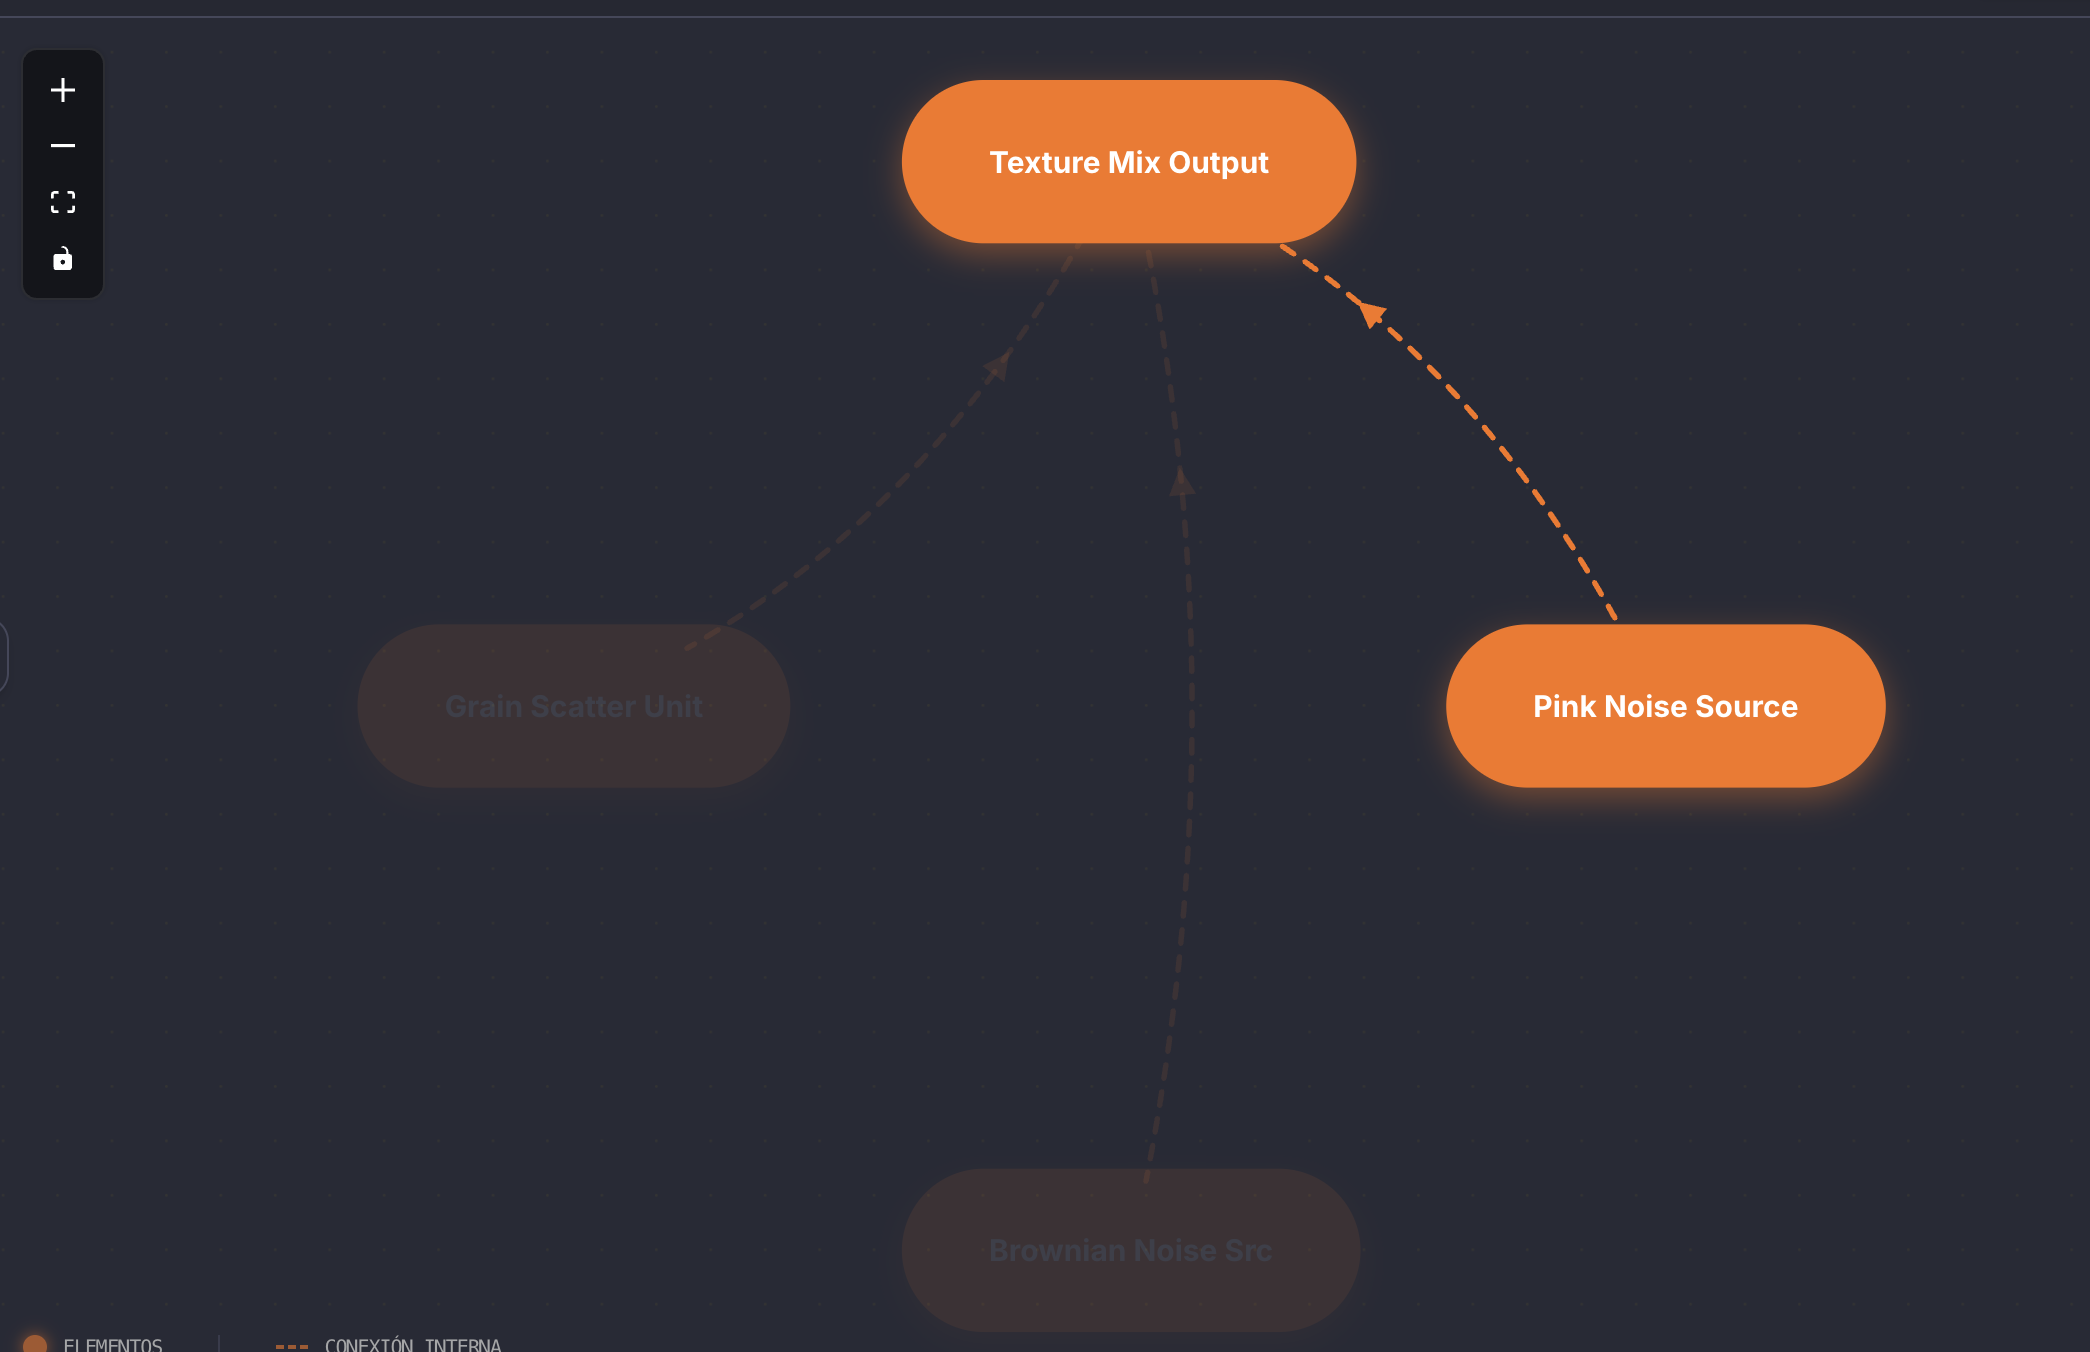
\includegraphics[width=\textwidth]{imagenes/05_analisis/19_visorGraficoMaquinaCimNodoPulsado.png}
    \caption{Inspección de las propiedades de los puertos y parámetros internos.}
\end{figure}

Al igual que en el nivel superior, existe un visor interactivo que mapea los bloques funcionales, puertos y conexiones internas que dotan de comportamiento al elemento musical conceptual.

\subsection{Gestión de Elementos de Máquina}

\begin{figure}[!ht]
    \centering
    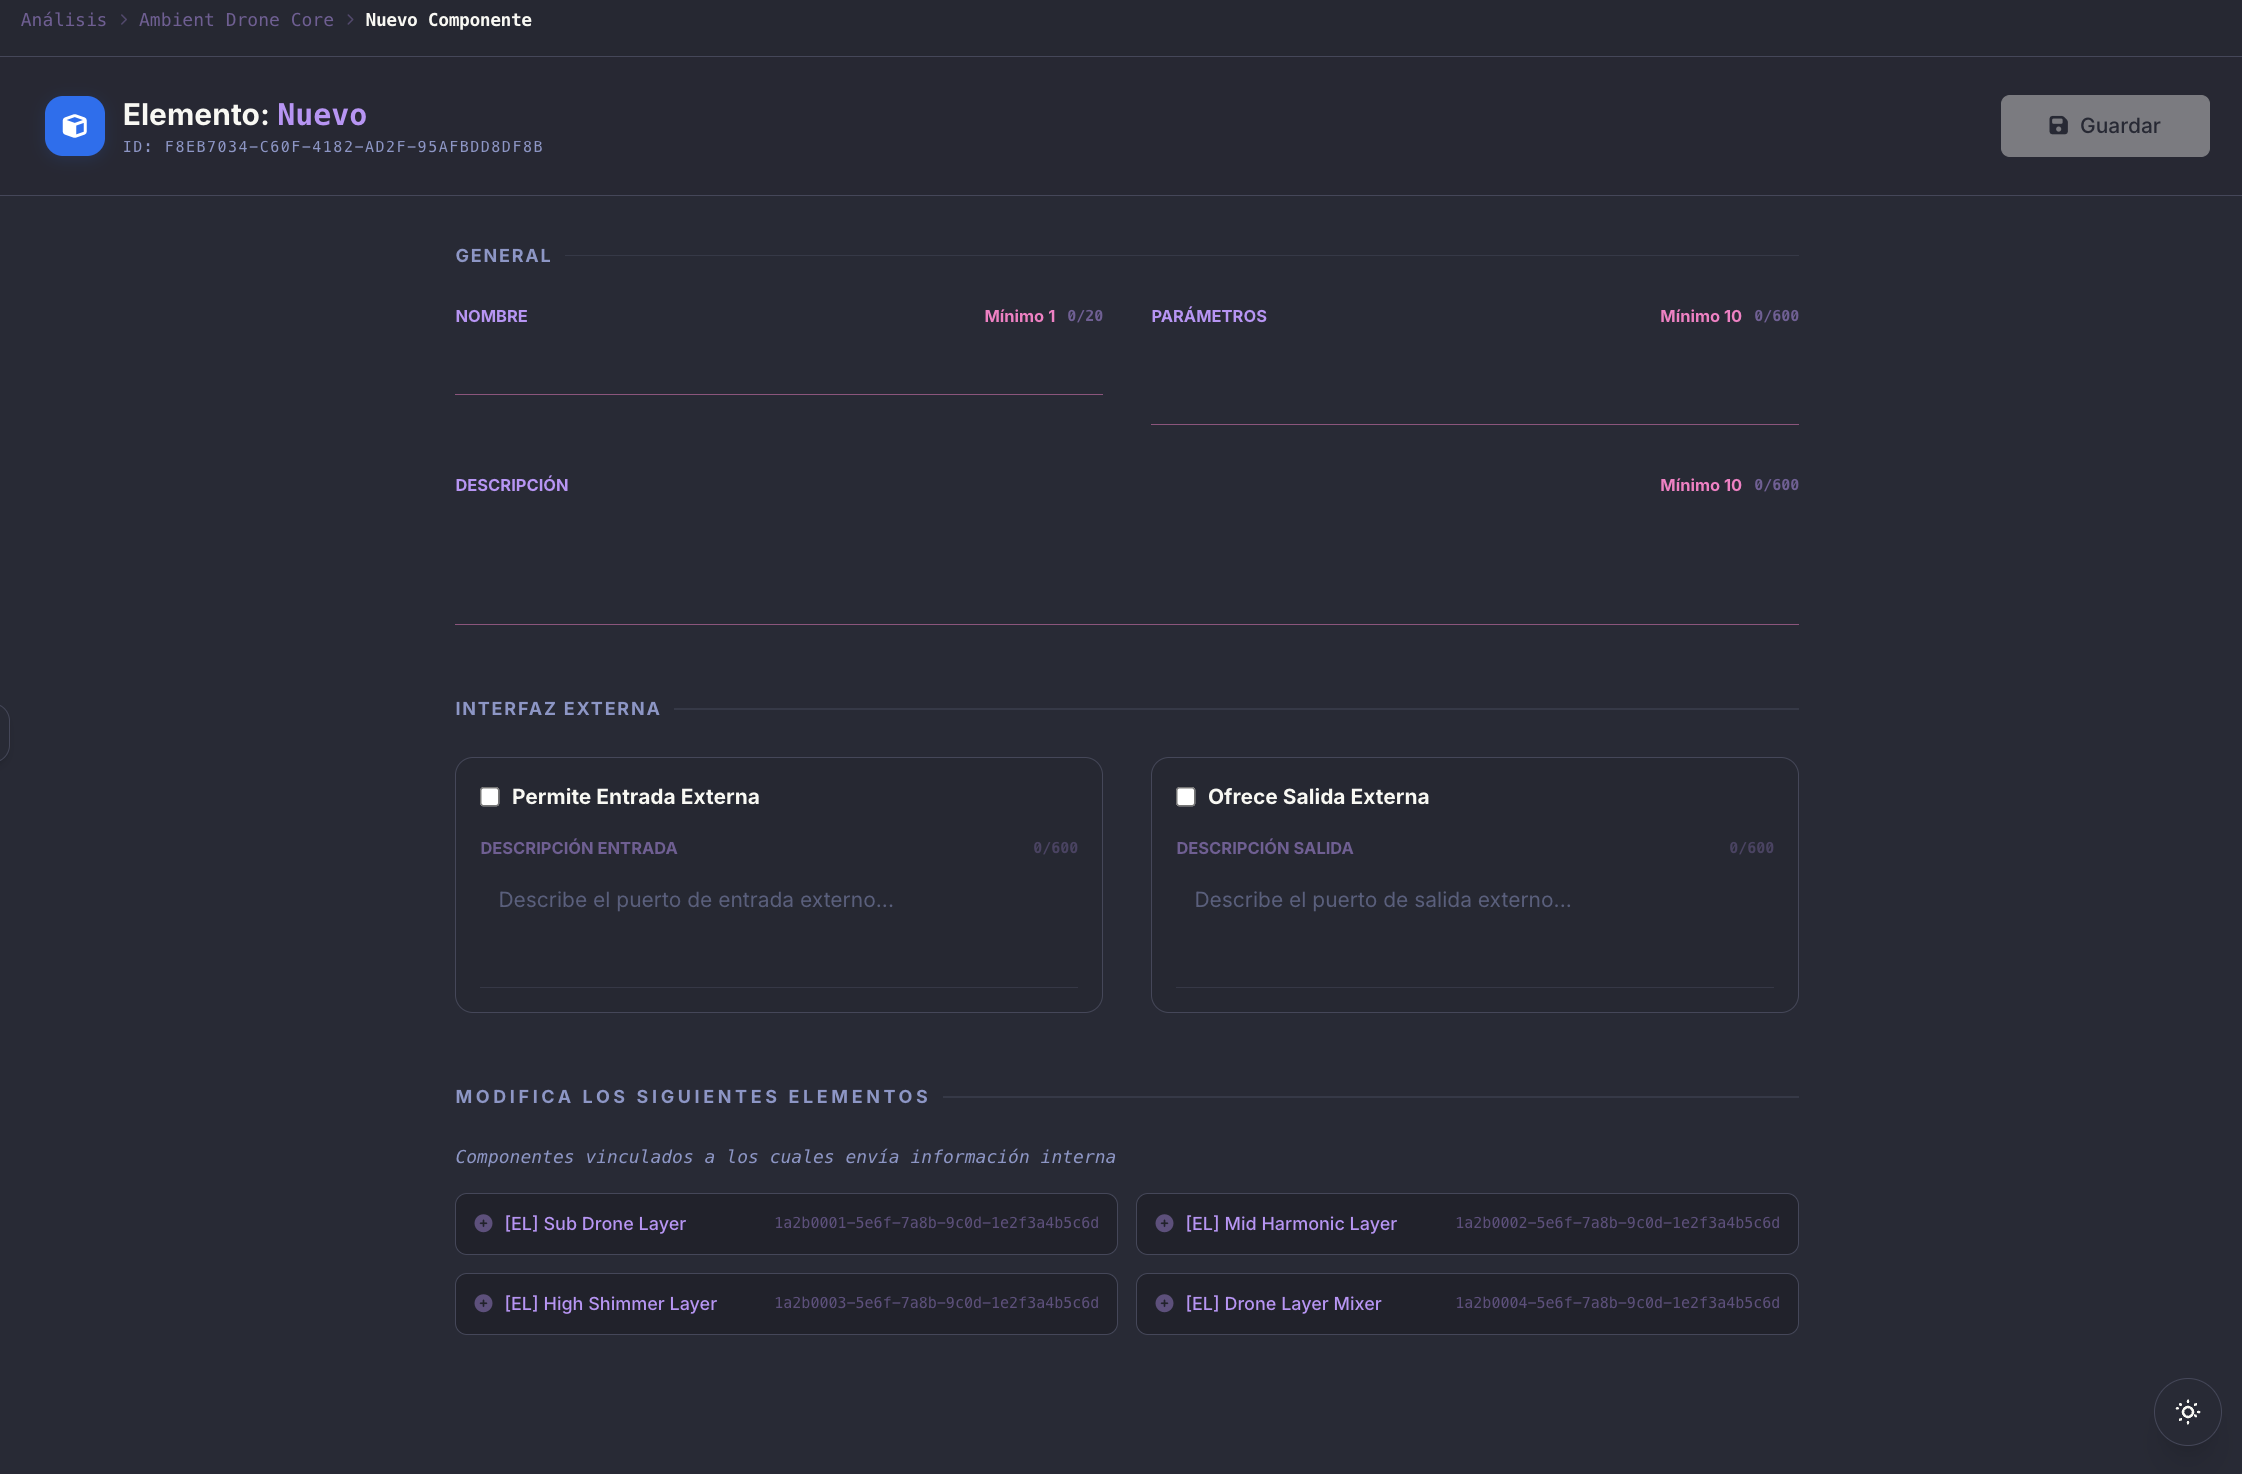
\includegraphics[width=\textwidth]{imagenes/05_analisis/20_formularioCrearElementoDeMaquinaCim.png}
    \caption{Formulario para la adición de nuevos elementos internos.}
\end{figure}

\begin{figure}[!ht]
    \centering
    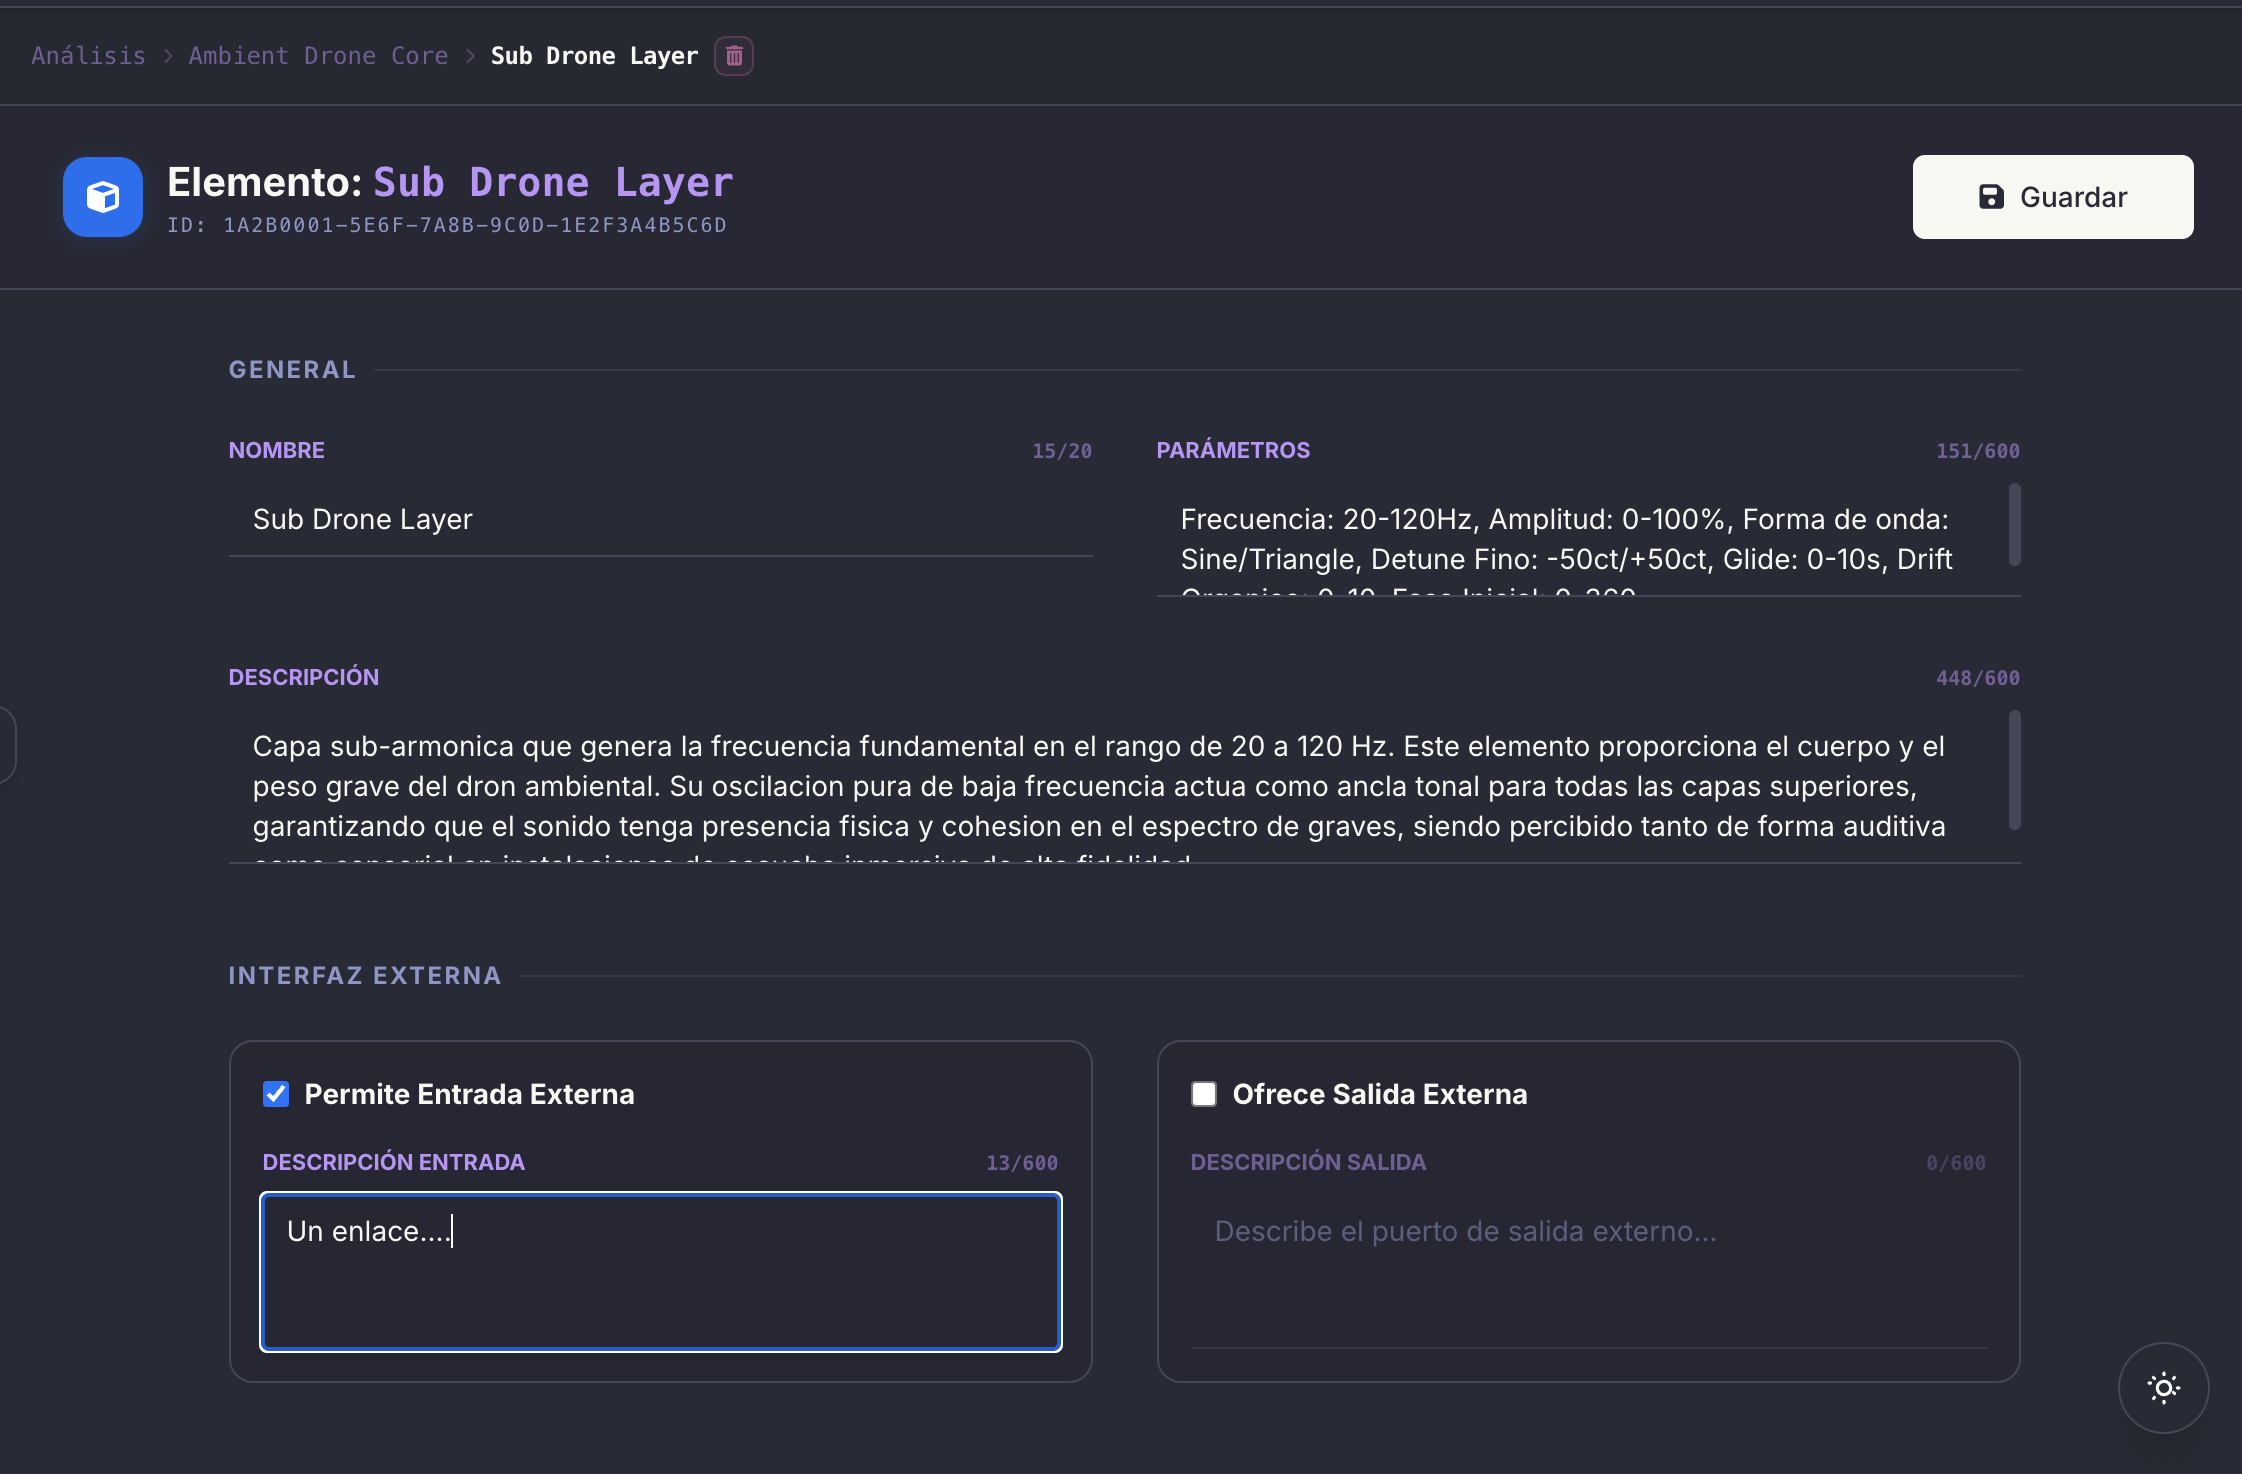
\includegraphics[width=\textwidth]{imagenes/05_analisis/21_formularioRellenoElementoMaquinaCim.png}
    \caption{Vista detallada de un elemento interno con su configuración completa.}
\end{figure}

El formulario de edición de elementos asiste en la asignación de atributos vitales (tipos, dominios, valores predeterminados) definidos por el modelo de datos \textit{CIM}.

\begin{figure}[!ht]
    \centering
    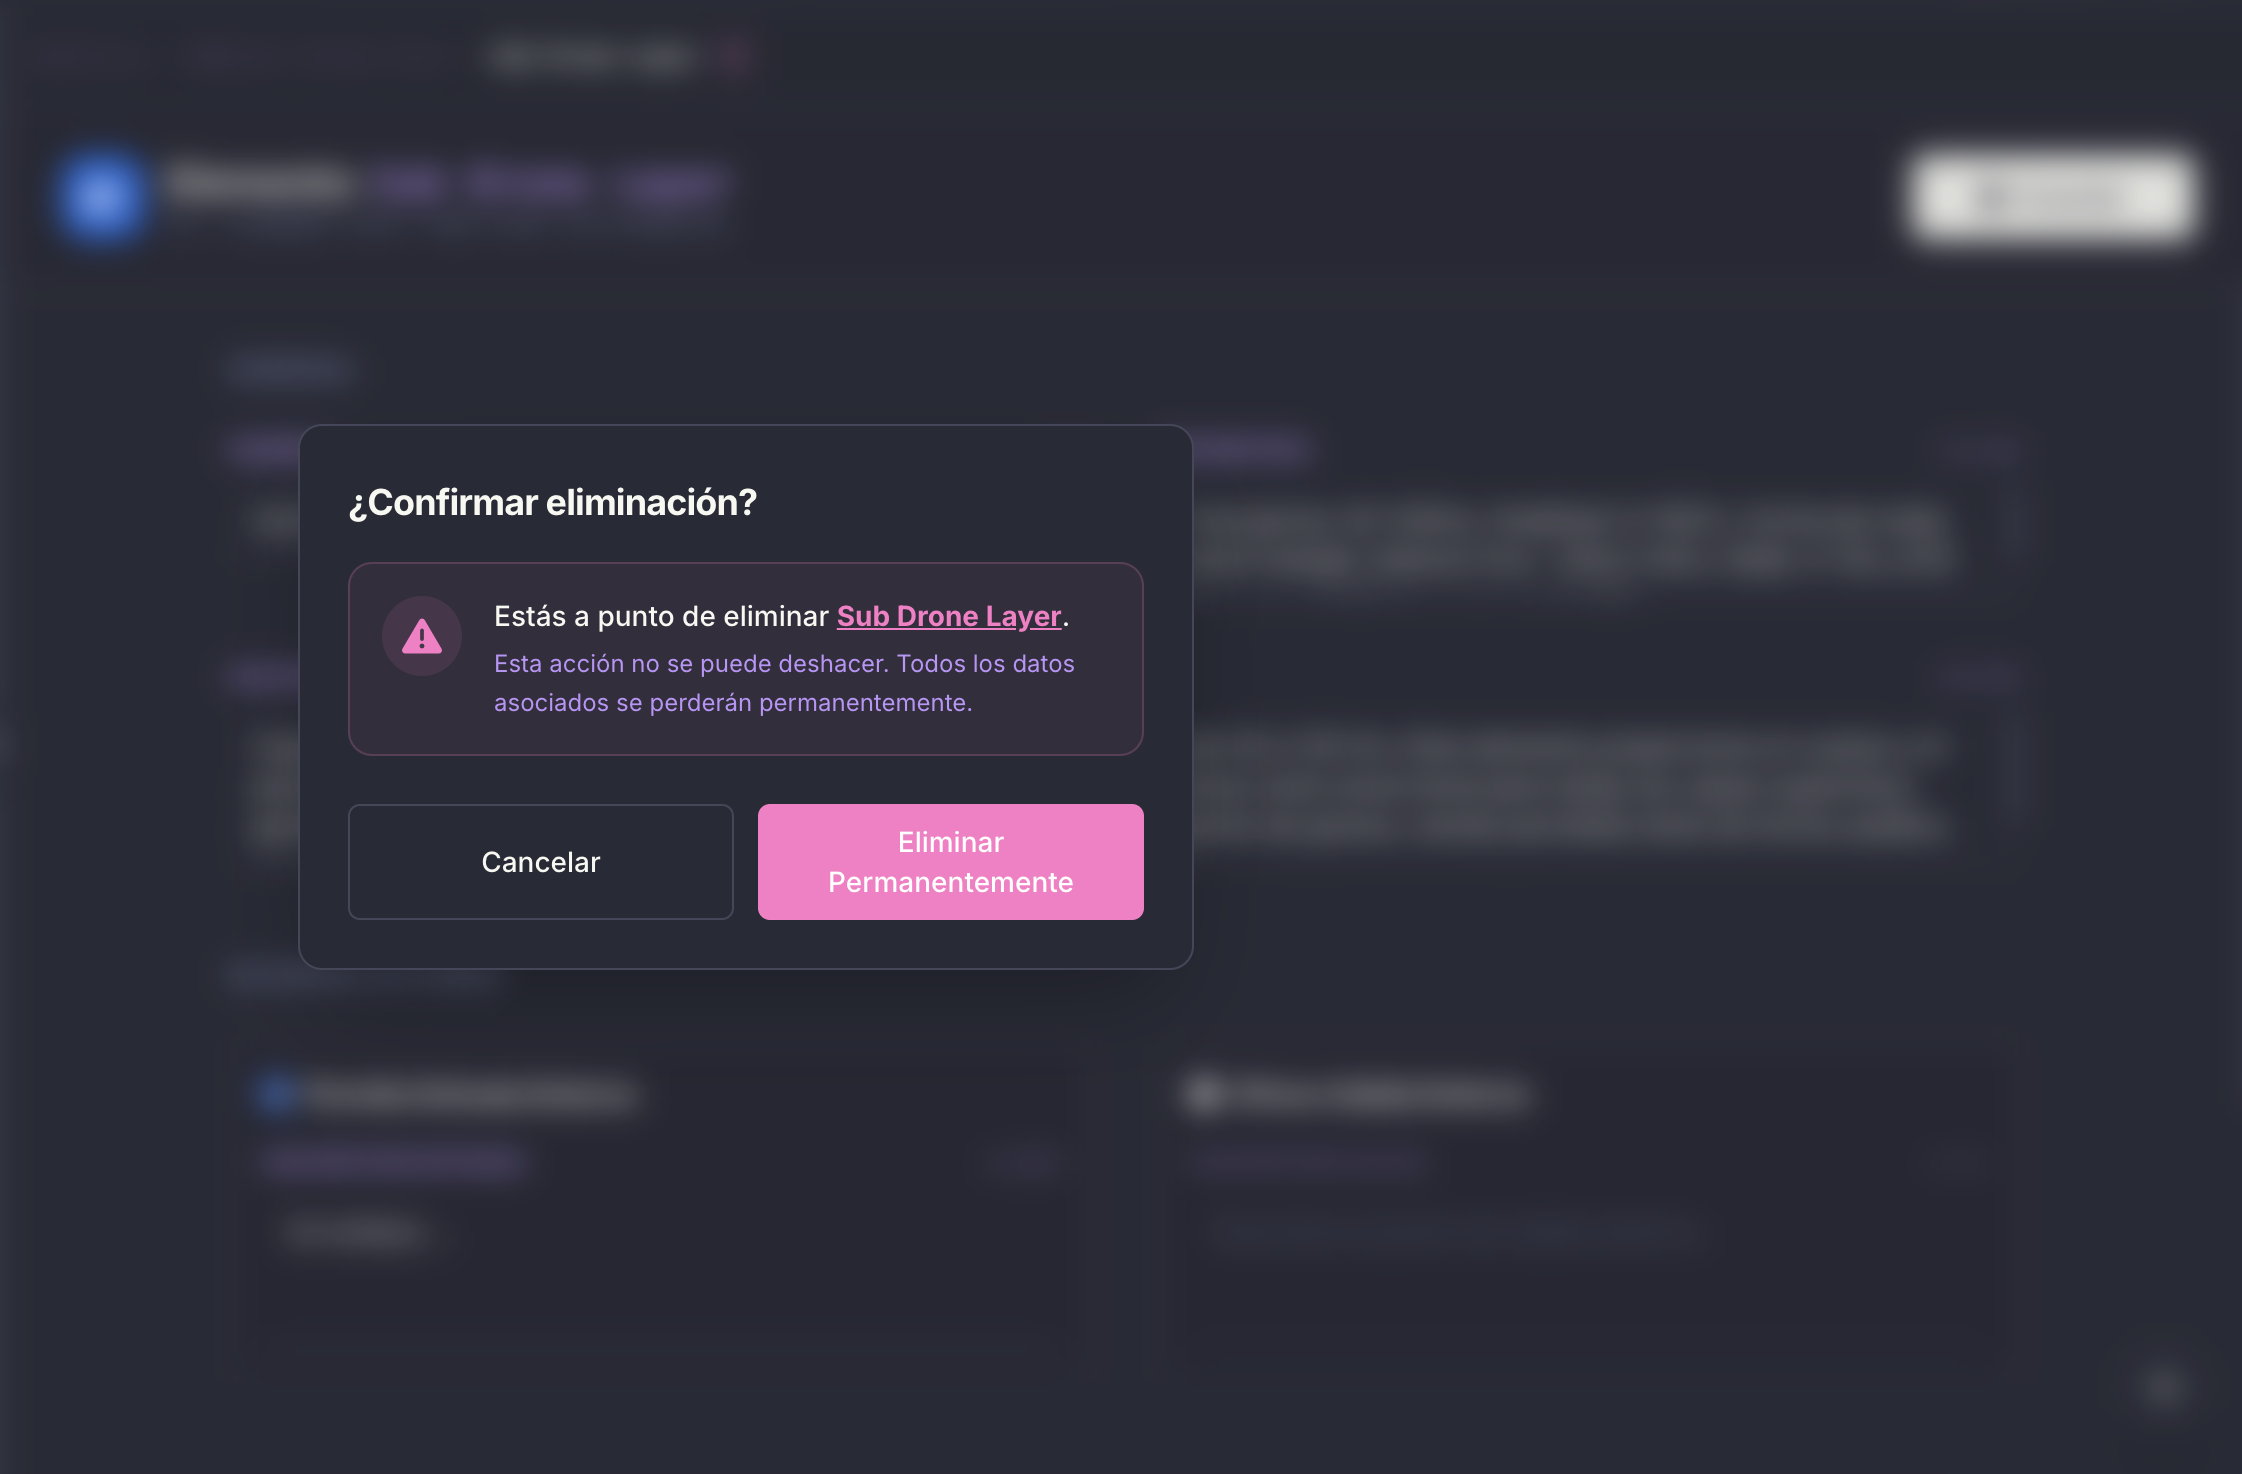
\includegraphics[width=0.6\textwidth]{imagenes/05_analisis/22_eliminarElementoMaquinaCim.png}
    \caption{Solicitud de confirmación para eliminar un componente interno.}
\end{figure}

\begin{figure}[!ht]
    \centering
    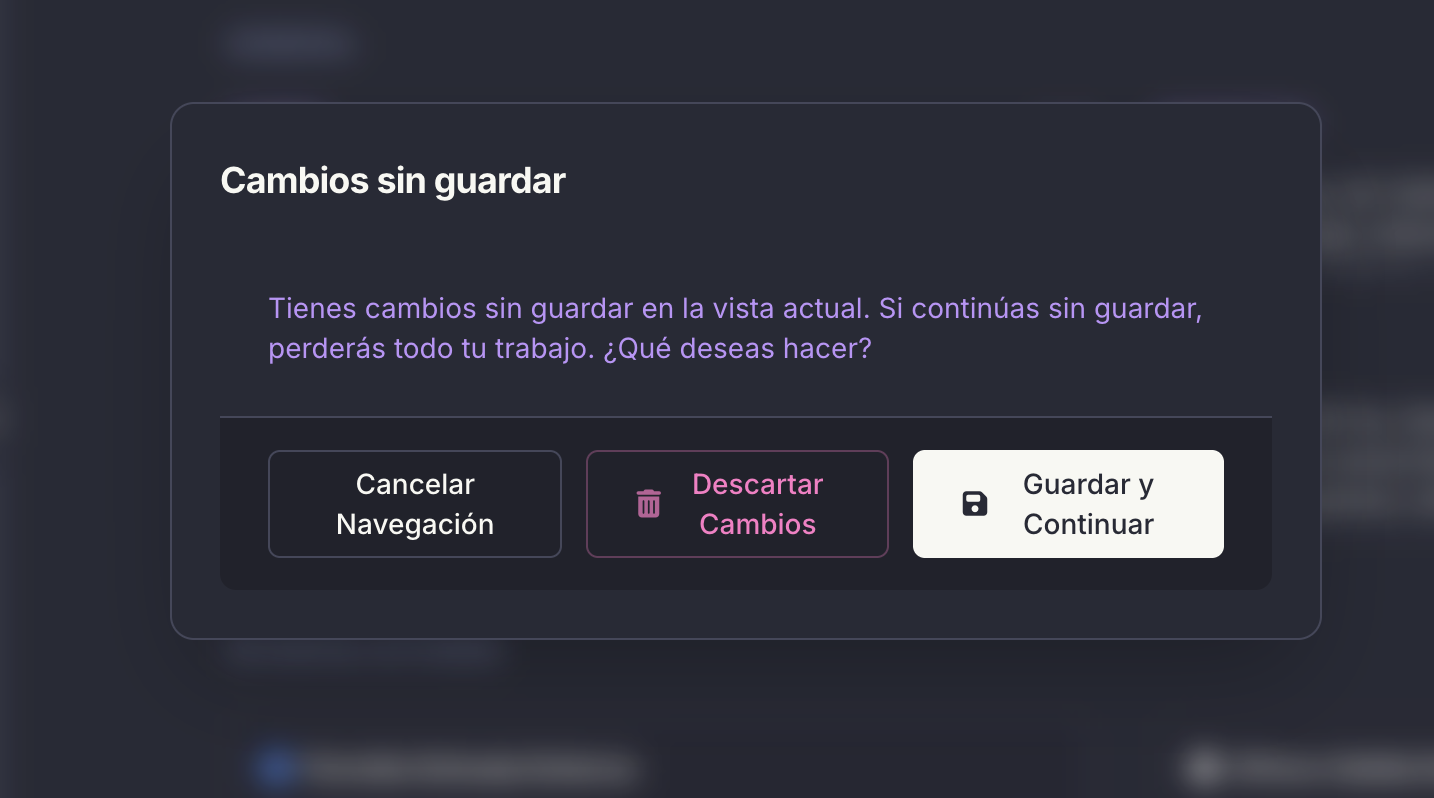
\includegraphics[width=0.6\textwidth]{imagenes/05_analisis/23_salirDeFromularioElemengtoMaquinaCimSinSalvar.png}
    \caption{Protección contra pérdida de datos al editar elementos de máquina.}
\end{figure}

La modificación de los interiores de la máquina está protegida mediante validaciones y cuadros de diálogo de confirmación, asegurando que las alteraciones estructurales (eliminaciones o abandonos no guardados) sean siempre acciones deliberadas del usuario.
